% Patched per referee assessment; baseline compiled from the user’s latest text.
\documentclass[aps,prd,onecolumn,superscriptaddress,nofootinbib]{revtex4-2}

% — Packages —
\usepackage[utf8]{inputenc}
\usepackage[T1]{fontenc}
\usepackage{lmodern}
\usepackage{amsmath,amssymb,bm,mathtools,amsthm}
\usepackage{graphicx}
\usepackage{adjustbox}
\usepackage{xcolor}
\usepackage{microtype}
\usepackage[unicode, pdfencoding=auto, psdextra]{hyperref}
\usepackage{enumitem}
\usepackage{tikz}
\usepackage{booktabs}
\usepackage{siunitx}
\sisetup{detect-all}
\usetikzlibrary{arrows.meta,positioning,fit,calc,shapes.geometric,shapes.multipart,backgrounds}

% — Colors for flowchart —
\definecolor{flowBlue}{HTML}{1F77B4}
\definecolor{flowPurple}{HTML}{9467BD}
\definecolor{flowGreen}{HTML}{2CA02C}
\definecolor{flowOrange}{HTML}{FF7F0E}
\definecolor{flowRed}{HTML}{D62728}
\definecolor{flowGray}{HTML}{7F7F7F}

% — Hyperref —
\hypersetup{
  colorlinks=true,
  linkcolor=blue,
  citecolor=blue,
  urlcolor=blue
}

% — PDF string sanitization —
\pdfstringdefDisableCommands{%
  \def\OmL{OmegaLambda}%
  \def\Omm{Omega m0}%
  \def\cgeo{cgeo}%
  \def\alphaM{alphaM}%
  \def\eps{epsilon}%
  \def\boxed#1{#1}%
  \def\mu{mu}%
  \def\alpha{alpha}%
  \def\alpha_M{alphaM}%
  \def\Omega_\Lambda{OmegaLambda}%
}

% — Math tweaks —
\allowdisplaybreaks

% — Macros —
\providecommand{\mpl}{M_{\rm P}}
\providecommand{\OmL}{\Omega_\Lambda}
\providecommand{\Omm}{\Omega_{m0}}
\providecommand{\cgeo}{c_{\rm geo}}
\providecommand{\alphaM}{\alpha_M}
\providecommand{\eps}{\varepsilon}
\providecommand{\be}{\begin{equation}}
\providecommand{\ee}{\end{equation}}
\providecommand{\bse}{\begin{subequations}}
\providecommand{\ese}{\end{subequations}}
\newcommand{\zenododoi}{10.5281/zenodo.TBD} % <– replace with final DOI before submission

% — Theorem-like environments —
\newtheorem{definition}{Definition}
\newtheorem{hypothesis}{Hypothesis}
\newtheorem{lemma}{Lemma}
\newtheorem{proposition}{Proposition}
\newtheorem{theorem}{Theorem}
\newtheorem{corollary}{Corollary}

\begin{document}

\title{Modular Response in Free Quantum Fields:\\
A KMS/FDT Theorem and Conditional Extensions}

\author{[clg]}
\affiliation{[Institutions]}
\date{}

\begin{abstract}
\textbf{Part I (Theoremic core, free/Gaussian Hadamard QFT).} We prove that, for small causal diamonds (CHM) in locally Hadamard states and within a safe window \(\epsilon_{\rm UV}\ll\ell\ll \min\{L_{\rm curv},\lambda_{\rm mfp},m_i^{-1}\}\), the MI/moment-kill projector isolates a finite \(\ell^4\) modular response with coefficient equal to its flat-space value; the projected KMS/FDT susceptibility is positive; and coarse-graining over the wedge family produces the universal weak-field prefactor \(5/12=(4/3)\times(5/16)\). The fractional KMS defect between CHM diamonds and half-spaces scales as \(\mathcal O((\ell/L_{\rm curv})^2)+\mathcal O((\ell H)^2)\). The QFT sensitivity is \(\beta=2\pi C_T I_{00}=0.02086\pm 0.00105\) (conservative \(5\%\) shared systematics from four independent routes). A scheme-invariant background relation \emph{suggests} \(\OmL=\beta\, f\,\cgeo\) \emph{conditional} on our coarse-graining and analyticity assumptions.

\smallskip
\textbf{Part II (Conditional extensions).} We separate \emph{definition} (flat-space \(\eps\) from modular response) from \emph{mapping}. Rather than impose the standard EFT-of-DE \(\alpha\)-basis, we adopt a quasi-static closure that keeps operational distances GR-like (no additional lensing coupling \(\Sigma\simeq 1\)) while modifying growth via \(\mu(\eps,s)=1/(1+\tfrac{5}{12}\eps\,s(x))\) with \(s(x)\) a local, covariant environment modulation derived from the action. We supply a frame-independence remark and an action-level realization of \(s(x)\). KMS/FDT positivity motivates an entropy-driven law \(d\eps/d\ln a\ge 0\) with a \emph{conditional} background budget \(\int \eps\,d \ln a=\OmL\). Cosmological illustrations (\(S_8\) band and \(H_0\) bounds) are \textbf{toy/illustrative} and propagate the \(\pm5\%\) \(\beta\) uncertainty; \emph{observed lensing amplitudes still reflect the altered growth}.

\smallskip
\textbf{Part III (Exploratory).} (i) An \emph{optional}, shock-selective \emph{optical} channel (Assumption D\(^{\prime}\)) reduces \(\Sigma\) only in high-shear shocked gas to address Bullet-type lensing offsets while preserving FRW distances. We retain a simple local saturating law in the text, and now provide a \emph{principled derivation path} from Schwinger–Keldysh (SK) hydrodynamics that makes \(\alpha_{\rm opt}\) a calculable function of ICM transport coefficients (App.~\ref{app:SK}). (ii) A compact thermodynamic interpretation of the projected modular response: a Clausius-like identity holds at working order in the MI/moment-kill channel, and the FRW budget may be viewed as a \emph{coarse-grained} Clausius normalization \emph{conditional} on our KMS\(\to\)FRW hypotheses. We clarify the relation to the Casini–Galante–Myers critique of Jacobson.
\end{abstract}

\maketitle

% ============================================================
\section*{Reader’s map: Part I (Theorem) vs.\ Part II (Conditional) vs.\ Part III (Exploratory)}
\noindent \textbf{Part I (Secs.~\ref{sec:scope}–\ref{sec:five-twelve}, Apps.~\ref{app:MI}–\ref{app:chm-kms-estimate}):} proven results for free/Gaussian Hadamard fields at working order.\\
\textbf{Part II (Secs.~\ref{sec:def-vs-map}–\ref{sec:data}, Apps.~\ref{app:fv}–\ref{app:microlocal}, \ref{app:entropic-proof}):} conditional extensions, Assumptions C \& D (stated), safe-window fraction, KMS\(\to\)FRW link, \emph{action-derived} environment modulation, entropic sketch, and toy/illustrative numerics with propagated uncertainties.\\
\textbf{Part III (Secs.~\ref{sec:lemmaDprime}, \ref{sec:thermo}, App.~\ref{app:SK}):} exploratory shock-selective optical response (Assumption D\(^{\prime}\)) with an SK/BRSSS derivation path and a thermodynamic interpretation (Clausius form in the projected channel; conditional FRW budget) and relation to CGM’s critique of Jacobson.

% ===============================
\section{Scope, Working Order, and Safe-Window Quantification (Part I)}
\label{sec:scope}

\paragraph{Working order and state class.} We work to \(\mathcal O(\ell^4)\) in the MI/moment-kill projector channel, treating curvature/contact terms as \(\mathcal O(\ell^6)\). States are locally Hadamard.

\paragraph{KMS applicability (CHM diamonds).} Exact BW KMS holds for half-spaces; CHM diamonds inherit it with fractional defect \(\mathcal O((\ell/L_{\rm curv})^2)+\mathcal O((\ell H)^2)\) (App.~\ref{app:chm-kms-estimate}).

\paragraph{Safe-window volume fraction.} Define a conservative admissible scale
\be
\label{eq:lmax}
\ell_{\max}(x)\equiv \zeta\,\min\Big\{L_{\rm curv}(x),\ \lambda_{\rm mfp}(x),\ m_i^{-1}(x)\Big\},\qquad \zeta=0.1.
\ee
Using Press–Schechter/Sheth–Tormen mass functions and NFW curvature proxies \(L_{\rm curv}^{-2}\sim (R_{abcd}R^{abcd})^{1/2}\) with substructure excision parameter \(\xi\), we estimate the comoving volume fraction \(f_V(\ell_{\min})=\mathrm{Vol}\{x:\,\ell_{\max}(x)>\ell_{\min}\}/\mathrm{Vol}_{\rm tot}\). A semi-analytic survey (App.~\ref{app:fv}) shows voids dominate \(f_V\), while dense cores lack a window; representative values at \(z\!\sim\!0\) for \(\ell_{\min}\in[1,100]\) pc are \(f_V\sim 0.6{-}0.95\) for \(\xi\in[0.2,0.5]\). This enters only as a domain-of-validity indicator.

\paragraph{Spectrum caveat.}
The admissible window \(\epsilon_{\rm UV}\ll \ell\ll\min\{L_{\rm curv},\lambda_{\rm mfp},m_i^{-1}\}\) is understood to apply to sectors that contribute at working order. Massive sectors with \(\ell\gg m_i^{-1}\) are exponentially suppressed and, after MI/moment–kill subtraction, do not re‑introduce lower moments or \(\ell^4\log\ell\) terms. Thus the \(\ell^4\) coefficient is dominated by massless/light fields while heavy fields decouple in this channel.

\paragraph{Angle invariance as a null test.} The continuous-angle product \(\mathcal C_\Omega=f(\theta)\,\cgeo(\theta)\) is analytic and \(\theta\)-independent; residuals are shown as a null check, not a precision claim.

% ===============================
\section{A2–KMS Theorem (Gaussian/Hadamard Sector)}
\label{sec:theorem}

\begin{theorem}[Projected modular response and positivity]\label{thm:proj-modresp}
Let \(\mathcal Q\) be a free (Gaussian) QFT on a globally hyperbolic spacetime and \(\rho\) a locally Hadamard state. For a causal diamond of radius \(\ell\) with \(\ell\ll L_{\rm curv}\) and the MI/moment-kill projector that cancels \(r^0\) and \(r^2\) moments, the MI-subtracted modular response obeys
\be
\delta\!\langle K_{\rm sub}\rangle=(2\pi C_T I_{00})\,\ell^4\,\delta\eps+\mathcal O(\ell^6),
\ee
with coefficient equal to the flat-space value. The retarded susceptibility \(\chi_{QK}\) in the projected channel is positive (FDT), and wedge averaging yields the universal weak-field prefactor \(5/12\). The fractional deviation from BW KMS is \(\mathcal O((\ell/L_{\rm curv})^2)+\mathcal O((\ell H)^2)\).
\end{theorem}

\begin{corollary}[Conditional background statement]\label{cor:background-cond}
Under the coarse-graining and analyticity assumptions of Sec.~\ref{sec:kms-frw}, the FRW zero mode \emph{suggests} the scheme-invariant relation
\(\OmL=\beta\,f\,\cgeo\) with \(\beta=2\pi C_T I_{00}\). We treat this as a conditional statement rather than a theorem.
\end{corollary}

% ===============================
\section{QFT Input: \texorpdfstring{$\beta=2\pi C_T I_{00}$}{beta} and Error Budget}
\label{sec:beta}
We evaluate \(\beta\) via four independent routes: (a) real-space CHM; (b) spectral/Bessel; (c) Euclidean time-slicing; (d) replica finite-difference. The spread is \(\lesssim 1\%\). We adopt a conservative
\be
\beta=0.02086\pm 0.00105 \quad (5\%~\text{shared systematics}).
\ee
Angle invariance is used as a null residual test.

\noindent Here \(C_T\) denotes the flat-space stress-tensor two-point normalization, e.g.
\(\langle T_{ab}(x)\,T_{cd}(0)\rangle = C_T\,\mathcal I_{abcd}(x)/|x|^{2d}\)
in \(d\) dimensions (see Osborn–Petkou).

\noindent\emph{Benchmark (convention).} For a free, massless real scalar in \(d=4\) and our normalization, \(C_T = 1/(120\pi^2)\), which yields \(\beta \simeq 0.02086\) via Eq.~\eqref{eq:eps-def}.

\noindent\textbf{Implementation consistency (note).} The normative constants used for the numerical reproductions are
\[
C_T=\frac{1}{120\pi^2},\qquad (\sigma_1,\sigma_2)=\Big(\tfrac{1}{2},2\Big),\qquad (a,b)=\Big(\tfrac{4}{5},\tfrac{1}{5}\Big),
\]
with the moment-kill identities enforced exactly (App.~\ref{app:MI}). Helper scripts (\texttt{beta\_methods\_v2.py}, \texttt{referee\_pipeline.py}) print these values alongside the computed \(I_{00}\) to prevent normalization drift.\footnote{In earlier development branches some convenience flags defaulted to alternate normalizations (e.g.\ \(C_T=3/\pi^4\)) and near-unity MI scales. These have been disabled in the archival runners; the paper’s conventions are authoritative.}

\noindent\textbf{Reproducibility (non‑circular).} We use a two–scale MI/moment‑kill subtraction with a top‑hat window on 3‑balls
\[
W_\ell(r)=\frac{3}{4\pi \ell^3}\,\Theta(\ell-r),\qquad
\mathcal{W}_\ell:=\int_{B_\ell}\!W_\ell-\;a\!\int_{B_{\sigma_1\ell}}\!W_{\sigma_1\ell}-\;b\!\int_{B_{\sigma_2\ell}}\!W_{\sigma_2\ell}.
\]
The two moment‑kill conditions (cancelling \(r^0\) and \(r^2\) for any smooth radial \(F\)) fix
\[
a+b=1,\qquad a\,\sigma_1^2+b\,\sigma_2^2=1
\ \ \Longrightarrow\ \
a=\frac{\sigma_2^2-1}{\sigma_2^2-\sigma_1^2},\quad
b=\frac{1-\sigma_1^2}{\sigma_2^2-\sigma_1^2}.
\]
In our runs we take
\[
(\sigma_1,\sigma_2)=\Big(\tfrac{1}{2},\,2\Big),\qquad (a,b)=\Big(\tfrac{4}{5},\,\tfrac{1}{5}\Big)=(0.8,0.2).
\]
With these weights the projected \(\ell^4\) coefficient evaluates to
\[
I_{00}=3.932017\ \ \text{(dimensionless)},
\]
so with \(C_T=1/(120\pi^2)\) one obtains \(\beta=2\pi C_T I_{00}=0.02086\) as quoted. The helper script \texttt{beta\_methods\_v2.py} echoes both \((a,b;\sigma_1,\sigma_2)\) and the numeric \(I_{00}\).

% ===============================
\section{Weak-Field Prefactor \texorpdfstring{$5/12$}{5/12}}
\label{sec:five-twelve}
The isotropic BW channel gives \(\langle T_{kk}\rangle=(1+w)\rho\) with UV \(w=1/3\Rightarrow 4/3\).
Averaging over CHM segments yields \(5/16\), so \(5/12=(4/3)\times(5/16)\).
Details in App.~\ref{app:five-twelve}.

% ============================================================
\section{Definition vs.\ Mapping (Part II; Conditional)}
\label{sec:def-vs-map}

\paragraph{Definition (flat-space QFT).}
\be
\label{eq:eps-def}
\delta\!\langle K_{\rm sub}(\ell)\rangle=\underbrace{(2\pi C_T I_{00})}_{\beta}\,\ell^4\,\delta\eps(x)+\mathcal O(\ell^6).
\ee

\paragraph{Mapping (constitutive; beyond the \texorpdfstring{$\alpha$}{alpha}-basis).}
We \emph{do not} impose the linear EFT-of-DE \(\alpha\)-parameter mapping at working order. Instead, we adopt a quasi-static closure that keeps operational distances GR-like while modifying growth:
\bse
\label{eq:qs-closure}
\be
\nabla^2\Phi \;=\; 4\pi G a^2 \rho_m \,\mu(\eps,s), \qquad
\mu(\eps,s)=\frac{1}{1+\tfrac{5}{12}\eps\,s(x)},
\ee
\be
\nabla^2\frac{\Phi+\Psi}{2} \;=\; 4\pi G a^2 \rho_m ,\qquad (\Sigma\simeq 1\ \text{on FRW and in laminar flows}).
\ee
\ese
Here \(s(x)\) is a local scalar built from curvature (Sec.~\ref{sec:env}); in FRW, Weyl \(=0\Rightarrow \chi_g=0\Rightarrow s=1\).
\emph{Beyond working order we make no stability claims absent an action; \(\mu(\varepsilon,s)\) serves as a falsifiable diagnostic with \(\Sigma\simeq 1\).}
Matter obeys the standard continuity and Euler equations. This closure preserves the Bianchi identity at working order because \(s(x)\) is a scalar; an action-level realization and frame‑independence are given below (Remark~\ref{sec:throttle-remark}). \emph{Optional Assumption D\(^{\prime}\) (Sec.~\ref{sec:lemmaDprime})} introduces a \emph{shock-selective} lensing modification \(\Sigma(x)<1\) localized to high-shear gas while keeping FRW \(\Sigma\simeq 1\).

\noindent\emph{Remark on lensing amplitude.} \(\Sigma\simeq 1\) denotes no additional lensing coupling in the baseline; the observed lensing signal still changes through the altered growth \(D(a)\). Under Assumption~D\(^{\prime}\), \(\Sigma\) may be reduced \emph{locally} in shocked gas (\(\mathcal S_{\rm shock}\gg 1\)) without affecting FRW.

\paragraph{EFT stub (derivation of \(5/12\)).}
At quasi-static, sub-horizon scales, a background variation \(\delta\ln M^2=\beta\,\delta\varepsilon\) rescales the Poisson coupling as \(G\!\to\!G_{\rm eff}=G/(1+\Delta)\) with \(\Delta\) fixed by the universal weak-field bookkeeping. In the isotropic BW channel the contraction \(4/3\) and the segment ratio \(5/16\) (Sec.~\ref{sec:five-twelve}) give \(\Delta=\tfrac{5}{12}\varepsilon\), hence
\be
\mu(\varepsilon,s)=\frac{G_{\rm eff}}{G}=\frac{1}{1+\tfrac{5}{12}\varepsilon\,s(x)},
\label{eq:eft-stub}
\ee
consistent with Eqs.~\eqref{eq:qs-closure}.

\paragraph{Trial action (outlook).}
A possible action-level route consistent with our closure is to consider an effective term that modulates \(M^2\) via the modular response,
\[
S_{\rm trial}=\int d^4x \,\sqrt{-g}\left[\frac{M^2}{2}R + \lambda\,(\delta\!\ln M^2)\,\mathcal{K}[g;\ell] + \cdots\right],
\]
where \(\mathcal K\) is a local covariant scalar capturing the projected channel at working order and \(\lambda\) a running coefficient. While only illustrative, this shows how \(\delta\!\ln M^2=\beta\,\delta\varepsilon\) could arise from an action (cf.\ \cite{Jacobson2016,Lashkari2014}).

\subsection{Frame-independence of throttling (remark)}
\label{sec:throttle-remark}
\emph{Throttling} here means the reduction of the effective gravitational coupling relative to GR caused by the background state variable \(\varepsilon(a)\) and a local environment factor \(s(x)\) that encodes curvature/inhomogeneity.
In the Jordan frame we take
\[
M_*^2(x,a)=M^2\!\left[1+\tfrac{5}{12}\,\varepsilon(a)\,s(x)\right],\qquad
s(x)=\frac{1}{1+(\chi_g/\chi_\star)^q}+\mathcal O\!\Big(\frac{R}{m_s^2}\Big),
\]
so the quasi-static Poisson law reads
\[
\nabla^2\Phi \simeq \frac{4\pi G a^2 \rho_m\,\delta}{1+\tfrac{5}{12}\,\varepsilon(a)\,s(x)}
\quad\Rightarrow\quad
G_{\rm eff}(x,a)=\frac{G}{1+\tfrac{5}{12}\,\varepsilon(a)\,s(x)}.
\]
Thus throttling is present everywhere, while its magnitude is amplitude–modulated by the local invariant \(\chi_g=\ell^2\sqrt{C_{abcd}C^{abcd}}\): in weak fields (\(\chi_g\!\ll\!\chi_\star\)) one has \(s\!\to\!1\) and the full background rescaling \(G_{\rm eff}=G/(1+\tfrac{5}{12}\varepsilon)\); in strong fields (\(\chi_g\!\gg\!\chi_\star\)) one has \(s\!\to\!0\) and \(G_{\rm eff}\!\to\!G\) (Solar–System compliance).

A conformal map to the Einstein frame,
\[
\tilde g_{\mu\nu}=\Omega^2 g_{\mu\nu},\qquad \Omega^2=1+\tfrac{5}{12}\,\varepsilon(a)\,s(x),
\]
renders \(M_*\) constant and shifts the same throttling into the matter coupling. To working order in our MI/moment-kill channel, gradients of \(\Omega\) and of \(\chi_g\) enter only at \(\mathcal O\!\big((\ell/L_{\rm curv})^2\big)\) and \(\mathcal O(R/m_s^2)\), consistent with the error budget in Eq.~\eqref{eq:chi-defect} and App.~\ref{app:chm-kms-estimate}; the observables of interest are frame–independent at this order: growth is governed by
\[
\mu(\varepsilon,s)=\frac{1}{1+\tfrac{5}{12}\,\varepsilon(a)\,s(x)},
\]
and distances remain GR-like (\(\Sigma\simeq 1\), \(c_T=1\)).\footnote{This remark complements Assumption~D (Sec.~\ref{sec:lemmaD}): the working-order modification resides in a state- and environment-dependent \(M_*^2\) with no additional lensing coupling. A failure would manifest as our falsifiers in Sec.~\ref{sec:program}, e.g.\ a significant GW/EM distance split or a persistent \(\ell^4\log\ell\) term.}

\noindent\emph{Scale-separation note.} The \emph{local} modular response enters gravity solely as a renormalization \(\delta\!\ln M_*^2=\beta\,\delta\varepsilon\) of the Planck mass; the Einstein equations then propagate this renormalization to cosmological scales through the standard gravitational coupling. No macroscopic quantum coherence or ad hoc coarse-graining is required, and the Jordan\(\leftrightarrow\)Einstein map above makes this statement frame-independent at working order.

A simple way to realize \(s(x)\) is as an auxiliary heavy scalar that minimizes a local potential
\[
\mathcal V(s;\chi_g)=\frac{M^2 m_s^2}{2}\left[s-\frac{1}{1+(\chi_g/\chi_\star)^q}\right]^2,
\]
so that the algebraic EOM enforces \(s=[1+(\chi_g/\chi_\star)^q]^{-1}+\mathcal O(R/m_s^2)\). Choosing \(m_s^2\!\gg\!H_0^2\) ensures adiabatic tracking.

\noindent\textbf{Constraints (working order).}
(i) Choose \(m_s^2\gg H_0^2\) so \(s(x)\) adiabatically tracks \([1+(\chi_g/\chi_\star)^q]^{-1}\) and the \(\mathcal O(R/m_s^2)\) offset is negligible.
(ii) The Planck-mass drift \(\alpha_M=d\ln M_*^2/d\ln a=\frac{(5/12)\,s\,d\varepsilon/d\ln a}{1+(5/12)\varepsilon s}\) is naturally small under our monotone \(\varepsilon(a)\).
(iii) In FRW, Weyl \(=0\) so curvature-weighted corrections vanish; in LSS they are \(\mathcal O\!\big((\ell/L_{\rm curv})^2\big)\).

\noindent \emph{Weak-field acceleration (toy/conditional; clarification).} Because \(s\!\to\!1\) in low curvature, the weak-field normalization implies a MOND-like scale
\be
a_0=\frac{5}{12}\,\OmL^2\,c\,H_0,
\ee
Using the baseline \(\OmL=0.685\) and \(H_0=70.9~\mathrm{km\,s^{-1}\,Mpc^{-1}}\), this gives \(a_0^{\rm eff}\approx 1.2\times 10^{-10}\,\mathrm{m\,s^{-2}}\) in the weak-field limit (\(s\simeq 1\));
and the effective \(a_0^{\rm eff}\) is \emph{enhanced} in weak-field regimes by the \emph{derived} \(s\!\to\!1\) (not imposed), while Solar–System compliance follows from \(s(\chi_\odot)\ll 1\) (Sec.~\ref{sec:env}). Pipeline values propagate the \(\pm 5\%\) uncertainty in \(\beta\).

% ===============================
\section{Covariant KMS \texorpdfstring{$\to$}{->} FRW Link and Error Control}
\label{sec:kms-frw}
Let \(s\) denote modular time with \(\beta_{\rm KMS}=2\pi/\kappa\) locally, where \(\kappa\) is the local boost surface gravity so that the approximate conformal Killing field \(\xi^a\) satisfies \(\xi^a\nabla_a=\kappa\,\partial_s\).
Averaging the retarded kernel over a comoving congruence of diamonds and reparametrizing \(s\mapsto \ln a\) induces the FRW background factor \(f\,\cgeo\); diffeomorphism covariance is preserved because the averaging functional depends only on local curvature scalars and the diamond foliation. The total fractional defect in the kernel obeys
\be
\label{eq:chi-defect}
\frac{\delta\chi}{\chi_{\rm BW}}=\mathcal O\!\Big((\ell/L_{\rm curv})^2\Big)+\mathcal O\!\big((\ell H)^2\big)
\ \ \approx\ \ 10^{-12}+10^{-18}
\ee
for \(\ell\!\sim\!10\,\mathrm{pc}\), \(L_{\rm curv}\!\sim\!10\,\mathrm{Mpc}\), \(H^{-1}\!\sim\!4\,\mathrm{Gpc}\).

\begin{proposition}[FRW budget identity (conditional; analyticity hypothesis)]
\label{prop:frw-budget}
Assume: (H1) locality and rapid decay of the spatially averaged, projected retarded kernel so that its reparametrization defines a distribution in \(\ln a\); (H2) adiabatic evolution through matter domination so that \(J(a)=ds/d\ln a\propto H(a)^{-1}\) varies slowly; (H3) preservation of KMS analyticity of the averaged kernel under the reparametrization \(s\!\to\!\ln a\); and (H4) negligible CHM vs.\ half-space deviation at working order (App.~\ref{app:chm-kms-estimate}). Then
\[
\Big\langle \!\int \chi^{\rm proj}_{QK}(a,a')\,d^3x \Big\rangle
= \beta\, f\, \cgeo\, \delta(\ln a-\ln a') + \ldots
\]
and integrating the entropy-driven evolution \(d\eps/d\ln a=\sigma(a)I(a)\ge0\) yields the coarse-grained identity
\be
\int_{a_i}^{1}\!\eps(a)\,d\ln a \;=\; \OmL \;=\; \beta\, f\,\cgeo,
\label{eq:budget}
\ee
used as a normalization under (H1)–(H4).
\end{proposition}
\noindent\emph{Operational diagnostic.} The routine \texttt{referee\_pipeline.py} reports a scalar residual \(R_{\rm nonloc}\equiv\sum_{i\neq 0}\big|\bar\chi^{\rm proj}(\Delta_i)\big|\,\Delta(\ln a)_i\) outside the contact bin; by default we take the central bin(s) with \(|\Delta(\ln a)|\le \Delta_0\) as ``contact''. Declare failure if \(R_{\rm nonloc}/\sigma_{\rm boot}>3\) \emph{and} the contact weight \(w_0<0.95\). Unless noted, uncertainties are quoted at 68\% CL from bootstrap resampling; the \(R_{\rm nonloc}/\sigma_{\rm boot}>3\) criterion corresponds to a conservative \(\sim\!3\sigma\) (two-sided) flag.

\paragraph{Rigor note.}
A full microlocal proof of (H3)—preservation of KMS analyticity under the coarse-grained reparametrization \(s\!\to\!\ln a\)—is deferred to future work in the spirit of Hollands–Wald~\cite{HollandsWald2001}.

\paragraph{Thermodynamic analogy (pointer).}
The entanglement first law suggests a Clausius-like analogy (Sec.~\ref{sec:thermo}), \emph{conditional} on (H1)–(H4), with MI projection avoiding CGM’s marginality issues (App.~\ref{app:microlocal}).

% ===============================
\section{Assumptions for Interacting Extensions at Working Order (Part II; stated and test criteria)}
\label{sec:proofs}

\subsection{Assumption C (stated; test criteria): Relative entropy \texorpdfstring{$\leftrightarrow$}{<->} canonical energy in the projected diamond}
\label{sec:lemmaC}

\noindent\textbf{Statement.} For a local algebra \(\mathcal A(B_\ell)\) of an interacting Hadamard QFT obeying the microlocal spectrum condition and time-slice axiom, the MI/moment-kill projected second variation of Araki relative entropy equals the canonical-energy quadratic form of the projected stress tensor, up to \(\mathcal O(\ell^6)\) remainders, with a positive-definite projected kernel \(\chi_{QK}^{\rm proj}\).

\smallskip
\noindent\textbf{Rationale (sketch).} (i) The second variation is the Bogoliubov–Kubo–Mori metric. (ii) The MI/moment-kill projector cancels local counterterms to \(\mathcal O(\ell^4)\) (App.~\ref{app:MI}), conjectured to persist in interacting Hadamard QFTs (App.~\ref{app:microlocal}). (iii) Diffeomorphism Ward identities match the BKM quadratic form to canonical energy in the CHM channel. (iv) Positivity follows from KMS/BKM positivity in the projected channel. A complete microlocal proof is left to future work.

\paragraph{Operational tests (pass/fail).}
\begin{itemize}[leftmargin=*,noitemsep,topsep=0pt]
\item \textbf{Positivity test (substrates):} The projected, integrated retarded kernel \(\int\!\chi^{\rm proj}_{QK}\,d^4x\,d^4x'\) is nonnegative in Gaussian chains (exact) and HQTFIM (numerical tolerance) (checked with \texttt{hqtfim\_capacity\_probe.py}, \texttt{gaussian\_capacity\_probe.py}).
\item \textbf{No-\(\ell^4\log\ell\) falsifier:} The MI/moment-kill channel exhibits no \(\ell^4\log\ell\) term. \emph{Fail} if a protected-operator contribution produces an \(\ell^4\log\ell\) trend.
\item \textbf{Plateau stability:} Varying MI windows leaves the residual plateau \(\sim\mathcal O(\ell^6)\) (verifiable with \texttt{beta\_methods\_v2.py}). \emph{Fail} if residuals scale as \(\ell^4\) after subtraction.
\item \textbf{BKM positivity (finite truncations):} In truncated QFTs, the BKM quadratic form for \(\delta K_{\rm sub}\) is positive definite (tested with \texttt{gaussian\_capacity\_probe.py}). \emph{Fail} if negative eigenmodes persist under refinement.
\end{itemize}

\subsection{Assumption D (stated; test criteria): Uniqueness of the \texorpdfstring{$M^2$}{M^2} coupling at working order}
\label{sec:lemmaD}

\noindent\textbf{Statement.} In the \(c_T\!=\!1\), \(\alpha_B\!=\!0\) EFT corner linearized about FRW, with isotropy, parity, and time-reversal, the only background scalar coupling that survives the MI/moment-kill projection at \(\mathcal O(\ell^4)\) and modifies the weak-field growth sector while keeping distances GR-like is \(\delta\ln M^2\); other diffeomorphism-invariant local scalars are projected out, forbidden by sector constraints, or curvature-suppressed by \(\mathcal O((\ell/L_{\rm curv})^2)\).

\smallskip
\noindent\textbf{Rationale (sketch).} Consider the most general local covariant functional at the required engineering dimension:
\be
\delta\mathcal L=\sqrt{-g}\left[a\,R+b\,R_{ab}R^{ab}+c\,\nabla^2 R+d\,\delta\ln M^2\,R
+ e\,\delta g^{00}+ f\,K\,\delta g^{00}+ \cdots\right],
\ee
\noindent where ``\(\cdots\)'' denote terms of higher engineering dimension (e.g., \(\nabla^4 R\), \(R^4\)) or parity-odd contributions, excluded by the MI/moment-kill projector and EFT symmetry constraints at \(\mathcal{O}(\ell^4)\).
Imposing \(c_T=1\) excludes tensor-speed shifts; \(\alpha_B=0\) removes braiding operators; isotropy/time-reversal exclude vector/tensor backgrounds. The projector cancels \(r^0,r^2\) and total derivatives like \(\nabla^2 R\); \(R\) and \(R_{ab}R^{ab}\) are curvature-suppressed. Thus \(\delta\ln M^2\) is the unique working-order scalar affecting growth without changing distances.

\paragraph{Operational tests (pass/fail).}
\begin{itemize}[leftmargin=*,noitemsep,topsep=0pt]
\item \textbf{GR-like distances:} EM/GW luminosity distances agree at working order, \(|d_L^{\rm GW}/d_L^{\rm EM}-1|\lesssim5\times10^{-3}\). \emph{Fail} if a lensing coupling \(\Sigma\neq1\) is required.
\item \textbf{Growth-only modification:} Large-scale growth follows \(\mu(\varepsilon,s)\) with \(\Sigma\simeq1\) and standard continuity/Euler equations. \emph{Fail} if background \(\alpha_M\) must vary appreciably to reproduce \(\mu\neq1\).
\item \textbf{Solar-System compliance:} Environment modulation \(s(\chi_g)\) suppresses deviations: \(s(\chi_\odot)\ll10^{-5}\) (Table~\ref{tab:compliance}). \emph{Fail} if planetary bounds are violated.
\item \textbf{Falsifier link:} Any of the falsifiers in Sec.~\ref{sec:program} triggers failure of Assumption D.
\end{itemize}

\subsection{Assumption D\texorpdfstring{$^{\prime}$}{’} (optional; shock-selective optical channel)}
\label{sec:lemmaDprime}

\noindent\textbf{Independence.} Parts I–II do not rely on D\(^{\prime}\): if D\(^{\prime}\) fails, the theoremic results, the conditional FRW mapping, and the baseline growth-only modification with \(\Sigma\simeq 1\) remain intact. D\(^{\prime}\) is an exploratory, \emph{local} optical response intended for merging clusters with strong shocks.

\smallskip
\noindent\textbf{Motivation and scope.} Bullet-type systems exhibit weak-lensing peaks offset from shocked X-ray gas. Our baseline (\(\Sigma\simeq 1\)) preserves distances and attributes changes to growth; however, to address local lensing morphology in strongly shocked gas, we posit a shock-selective lensing response that leaves FRW and laminar flows untouched.

\smallskip
\noindent\textbf{Local, saturating law (predictive summary).} Let \(u^\mu\) be the baryon four-velocity and \(\sigma_{\mu\nu}\) the symmetric, trace-free shear. Define the shock indicator \(\mathcal S_{\rm shock}=\ell^2\sigma_{\mu\nu}\sigma^{\mu\nu}\ge 0\). We summarize the optical response by the purely local, saturating form
\be
\label{eq:sigmalocal}
\Sigma(x)\;\simeq\;1\;-\;\alpha_{\rm opt}\,\frac{\mathcal S_{\rm shock}(x)}{1+\mathcal S_{\rm shock}(x)},\qquad 0<\alpha_{\rm opt}<1,
\ee
so that \(\Sigma\to1-\alpha_{\rm opt}\) in strong shocks and \(\Sigma\to1\) away from shocks. The growth coupling \(\mu(\varepsilon,s)\) is unchanged; FRW and laminar flows have \(\mathcal S_{\rm shock}\approx 0\Rightarrow \Sigma\simeq 1\).

\paragraph{Transport-theory anchoring (SK/BRSSS link; derivation in App.~\ref{app:SK}).}
In viscous hydrodynamics (BRSSS) the anisotropic stress obeys
\[
\pi^{\mu\nu}+\tau_\pi\,u^\alpha\nabla_\alpha \pi^{\mu\nu}
=2\eta\,\sigma^{\mu\nu}+\lambda_1\,\sigma^{\langle\mu}{}_{\lambda}\sigma^{\nu\rangle\lambda}+\cdots,
\]
with \(\eta,\tau_\pi,\lambda_1\) fixed by Kubo formulas. In the cluster quasi-static limit (\(\omega\tau_\pi\ll 1\)) this reduces to \(\pi^{\mu\nu}\approx 2\eta\,\sigma^{\mu\nu}+\lambda_1\,\sigma^{\langle\mu}{}_{\lambda}\sigma^{\nu\rangle\lambda}\), which sources \((\Phi+\Psi)\) in the lensing equation. Matching to Eq.~\eqref{eq:sigmalocal} yields a \emph{computable} map
\be
\alpha_{\rm opt}\equiv \alpha_{\rm opt}(\eta,\tau_\pi,\lambda_1;T,n_e,B,\dots),
\qquad
\kappa_{\rm opt}\sim \frac{2\eta}{\rho_{\rm gas}\,c_s\,\ell}+\frac{\lambda_1}{\rho_{\rm gas}\,\ell^2}+\cdots,
\label{eq:alphaopt-map}
\ee
up to order-unity geometry factors (App.~\ref{app:SK}). Thus \(\alpha_{\rm opt}\) is \emph{not} a free fit-parameter in principle; it is determined by ICM transport.

\paragraph{Range and back-of-the-envelope calibration.}
In projected convergence, the local gas contribution scales as \(\kappa_{\rm gas}^{\rm eff}\!=\!\Sigma\,\kappa_{\rm gas}\).
To relocate the convergence peak from the shocked gas toward the collisionless galaxies in Bullet-like systems (offsets \(\sim\!200\) kpc; \cite{Clowe2006}), one needs \(\kappa_{\rm gas}^{\rm eff}\lesssim(0.2\text{--}0.4)\,\kappa_{\rm tot}\) within the shock sheet. For strong shocks \(\mathcal S_{\rm shock}\!\gg\!1\), Eq.~\eqref{eq:sigmalocal} gives \(\Sigma\simeq 1-\alpha_{\rm opt}\); thus \(\alpha_{\rm opt}\simeq 0.6\text{--}0.8\) suppresses the gas lensing weight by \(60\text{--}80\%\) where needed, while leaving FRW and unshocked regions (\(\mathcal S_{\rm shock}\!\ll\!1\)) essentially unmodified (\(\Sigma\simeq 1-\alpha_{\rm opt}\mathcal S_{\rm shock}\approx 1\)). This range is consistent with Mach \(\mathcal M\simeq 2\text{--}3\) shocks inferred from X-ray edges \cite{Markevitch2002}.

\paragraph{Operational predictions and falsifiers (Bullet-type tests).}
\begin{itemize}[leftmargin=*,noitemsep,topsep=0pt]
\item \textbf{Shock tracking (A):} The lensing suppression should spatially correlate with X-ray shock edges (temperature/surface-brightness jumps) and radio relics (tracing high-\(\sigma^2\) regions) \cite{Markevitch2002,vanWeeren2019}.
\item \textbf{Time evolution (B):} As shocks dissipate, \(\mathcal S_{\rm shock}\downarrow\) and \(\Sigma\to1\); convergence centroids drift back toward gas on the shock-cooling timescale.
\item \textbf{Mach-number scaling (C):} Lower-Mach mergers show smaller centroid offsets at fixed gas mass (cf.\ Bullet vs.\ Abell 520 \cite{Mahdavi2007}).
\item \textbf{Selectivity (D):} No suppression in unshocked or laminar gas; failure if convergence deficits appear where \(\mathcal S_{\rm shock}\approx 0\).
\end{itemize}

\paragraph{Safety checks.} \(c_T=1\) (no curvature-derivative couplings), FRW \(\Sigma\simeq1\) (\(\sigma_{\mu\nu}=0\)), Solar System unaffected, and the integrated GW/EM split remains \(\ll 10^{-3}\) since the effect is cluster-local. Positivity is manifest from the squared potential in App.~\ref{app:optics-details}.

\vspace{1ex}

% ===============================
\section{Entropy-Driven \texorpdfstring{$\varepsilon(a)$}{epsilon(a)} and Growth (Conditional)}
\label{sec:epsilon}

\paragraph{KMS/FDT positivity.}
Let \(\hat Q\) be the boost-energy flux and \(\chi_{QK}^{\rm proj}\) the retarded kernel in the projected channel. Then
\be
\frac{d\eps}{d\ln a}=\sigma(a)\,\mathcal I(a),\qquad \sigma(a)\ge 0,\ \ \mathcal I(a)\ge 0,\qquad
\int \eps\,d\ln a=\OmL=\beta\,f\,\cgeo.
\ee
A preliminary derivation with intermediate steps in App.~\ref{app:entropic-proof} details \(d\varepsilon/d\ln a \ge 0\) from Araki relative entropy, supporting the use of \(\mu(\varepsilon,s)\).

\paragraph{Fixed-point with growth.}
The growth factor \(D(a)\) satisfies
\be
\label{eq:growth-ode}
\frac{d^2 D}{d(\ln a)^2}
+\Big(2+\frac{d\ln H}{d\ln a}\Big)\frac{dD}{d\ln a}
-\frac{3}{2}\,\Omega_m(a)\,\mu(\eps(a),s)\,D=0,\qquad
\mu(\eps,s)=\frac{1}{1+\tfrac{5}{12}\eps\,s}.
\ee

\paragraph{Variational bounds (extremals).}
Convex-order arguments imply late-loaded \(\eps(a)\) minimizes \(S_8\) and early-loaded maximizes it, under monotonicity and budget. We therefore report an \(S_8\) \emph{band} bracketed by these extremals; any illustrative kernel (e.g., logarithmic exposure) must lie within the band.

\noindent\emph{Quantified extremals (illustrative).} In our baseline cosmology and for monotone \(\varepsilon(a)\) satisfying the budget \eqref{eq:budget}, late-loaded profiles give \(S_8\simeq 0.76\) while early-loaded profiles give \(S_8\simeq 0.82\); both inherit a \(\pm 0.008\) envelope from the \(\beta\) uncertainty propagated through Eq.~\eqref{eq:growth-ode}.

% ===============================
\section{Environment Modulation from Action and Calibration}
\label{sec:env}

\paragraph{Units and conventions.}
We work in geometric units \(G=c=1\). When inserting SI values we convert masses via \(M\mapsto GM/c^2\); this keeps the curvature scalar \(\chi_g=\ell^2\sqrt{C_{abcd}C^{abcd}}\) dimensionless.

\paragraph{Action-derived modulation.}
We define
\be
s(x)=\frac{1}{1+(\chi_g/\chi_\star)^q}+\mathcal O\!\Big(\frac{R}{m_s^2}\Big),\qquad \chi_g\equiv \ell^2\sqrt{C_{abcd}C^{abcd}},
\ee
as the algebraic EOM solution of a heavy auxiliary field minimizing
\be
\mathcal V(s;\chi_g)=\frac{M^2 m_s^2}{2}\left[s-\frac{1}{1+(\chi_g/\chi_\star)^q}\right]^2,\qquad m_s^2\gg H_0^2,
\ee
so \(s\!\to\!1\) in weak curvature (\(\chi_g\!\ll\!\chi_\star\)) and \(s\!\to\!0\) in strong curvature (\(\chi_g\!\gg\!\chi_\star\)). In FRW, Weyl\(=0\) so \(\chi_g=0\Rightarrow s=1\).
This \(s(x)\) enters \(\mu(\varepsilon,s)=1/\!\big[1+(5/12)\varepsilon\,s\big]\) (Sec.~\ref{sec:def-vs-map}).

\paragraph{Calibration example (Solar System).}
For a Schwarzschild source the Weyl invariant obeys \(\sqrt{C^2}=\sqrt{48}\,M/r^3\) in geometric units, with \(M=GM/c^2\) when using SI inputs. Taking \(\ell=10\,\mathrm{pc}\), \(r=1\,\mathrm{AU}\), and \(M_\odot\simeq 1.477\,\mathrm{km}\), we find
\[
\chi_\odot \equiv \ell^2 \, \sqrt{48}\,\frac{M_\odot}{r^3} \approx 2.9\times 10^{5}.
\]
Imposing \(s(\chi_\odot)\le \epsilon_{\rm SS}=10^{-5}\) with \(q=2\) implies
\[
\chi_\star \lesssim \chi_\odot\,\epsilon_{\rm SS}^{1/2} \approx 9.2\times 10^{2}.
\]
A representative choice \(\chi_\star=900\), \(q=2\) then yields \(s(\chi_\odot)\approx 9.6\times 10^{-6}\), while leaving cosmological environments (\(\chi_g\ll\chi_\star\)) essentially unsuppressed (\(s\simeq 1\)). For transparency we report a small compliance table:

\begin{table}[t]
\centering
\caption{Solar–System compliance of the action-derived modulation \(s(\chi_\odot)\) at \(\ell=10\,\mathrm{pc}\), \(r=1\,\mathrm{AU}\) (Schwarzschild).}
\label{tab:compliance}
\begin{tabular}{lcccc}
\toprule
$\chi_\star$ & 1200 & 1000 & 900 & 800 \\
\midrule
$s(\chi_\odot;\,q{=}2)$ & $1.7\times 10^{-5}$ & $1.18\times 10^{-5}$ & $9.6\times 10^{-6}$ & $7.6\times 10^{-6}$ \\
\bottomrule
\end{tabular}
\end{table}

\paragraph{Phenomenology and alternatives.}
The choice \(s=[1+(\chi_g/\chi_\star)^q]^{-1}\) with \(q=2\) is a simple, Solar–System–compliant solution. We have also tested \textbf{alternative envelopes}, such as an exponential decay \(s_{\exp}(\chi_g)=\exp[-(\chi_g/\chi_\star)^p]\) (with \(p\!\sim\!1\text{--}2\)) and variants based on alternative curvature scalars (e.g., using \(R_{abcd}R^{abcd}\) proxies). Each corresponds to a different target in \(\mathcal V(s;\chi_g)\) and yields similar weak-/strong-field limits; quantitative differences appear mainly in the transition region and are constrained by data. These options are exposed in \texttt{cosmology\_runner.py} (see the \texttt{--s-form} and \texttt{--s-params} toggles), which we use for robustness checks. The power-law envelope used here should thus be regarded as a representative compliance function.

\subsection{BAO growth modulation (toy)}
The entropy-driven \(d\varepsilon/d\ln a \geq 0\) (App.~\ref{app:entropic-proof}) suggests BAO peak growth via near-GR reversion (e.g., \(d_L^{\rm GW}/d_L^{\rm EM}\approx 0.995\)) and lower \(g\) off-peak due to \(\mu(\varepsilon,s)\). A toy model with \(\chi_g\) sweeps (Sec.~\ref{sec:data}, \texttt{s8\_hysteresis\_run.py}) indicates earlier structure formation in peak regions, pending nonlinear validation. Quantitatively, \texttt{s8\_hysteresis\_run.py} yields a near-peak boost in \(D(a)\) of \(\sim 1\text{--}2\%\) with a compensating off-peak suppression (cf.\ growth parametrizations in \cite{BelliniSawicki2014}).

% ===============================
\section{Observational Illustrations (Illustrative under Secs.~\ref{sec:kms-frw}, \ref{sec:epsilon}; Uncertainty Propagated)}
\label{sec:obs}

\paragraph{Hubble ladder bounds (toy).}
Assuming the conditional background relation \(\OmL=\beta f\cgeo=0.685\pm 0.034\) and under the assumptions of Secs.~\ref{sec:kms-frw} and \ref{sec:epsilon}, the previously quoted illustrative shifts \(H_0: 73.0\to 71.18\) (uncapped SN) and \(\to 70.89\) (capped SN+Cepheid) acquire \(\pm 0.17~\mathrm{km\,s^{-1}\,Mpc^{-1}}\) systematic envelopes from \(\beta\), reported as
\be
H_0^{\rm toy}=\{71.18\pm 0.17,\ \ 70.89\pm 0.17\}\ \ \mathrm{km\,s^{-1}\,Mpc^{-1}}.
\ee

\paragraph{\(S_8\) band (toy).}
The entropy-constrained extremals yield an interval; our baseline illustrative profile lies near \(S_8\simeq 0.788\), with an inherited \(\pm 0.008\) envelope from \(\beta\). We report an \(S_8\) band rather than a fit, and distances remain GR-like. Allowing modest non-monotonic \(\varepsilon(a)\) histories can widen the band by \(\sim 3\text{--}5\%\).

\paragraph{Merging clusters (optional D\(^{\prime}\); exploratory).}
For shock Mach numbers \(\mathcal M\sim 2\text{--}3\) we expect \(\mathcal S_{\rm shock}\gtrsim \mathcal O(1\text{--}5)\) across the shock sheets; with \(\alpha_{\rm opt}\approx 0.6\text{--}0.8\) in Eq.~\eqref{eq:sigmalocal} this yields \(\Sigma_{\rm gas}\sim 0.2\text{--}0.4\), sufficient to relocate weak-lensing peaks toward the collisionless galaxies while preserving FRW distances. The predicted centroid offsets (\(\sim 200\) kpc) and shock strengths are consistent with Bullet Cluster observations \cite{Clowe2006,Markevitch2002}; radio relic/shock correlations provide an independent tracer of the high-shear regions \cite{vanWeeren2019}. Comparative systems (e.g., Abell 520) offer additional tests of the Mach-scaling prediction \cite{Mahdavi2007}.

% ===============================
\section{Structural Checks (Algebraic; Not 4D Surrogates)}
\label{sec:substrates}
HQTFIM and Gaussian chains confirm the algebraic ingredients (first-law channel, constant+log trend, vanishing plateau after subtraction, and positivity in the projected kernel). They are \emph{not} curved 4D surrogates.

% ===============================
\section{Proof Program Status and Falsifiers}
\label{sec:program}
\textbf{Lemma A} (diamond KMS control): scaling proven, sharp bounds left to microlocal analysis. \textbf{Lemma B} (projector universality): established. \textbf{Assumption C} and \textbf{Assumption D}: stated here with rationale; proofs deferred (Secs.~\ref{sec:lemmaC}, \ref{sec:lemmaD}). \textbf{Assumption D\(^{\prime}\)} (shock-selective optical channel): exploratory extension for merging clusters (Sec.~\ref{sec:lemmaDprime}; derivation path in App.~\ref{app:SK}). \textbf{Lemma E} (FDT positivity): follows from BKM positivity. \textbf{Lemma F} (geometric \(5/12\)): derived.\\
\textbf{Lemma G (Nonlinear validation)}: Initial Gadget-4 runs are complete (baseline resolution; \texttt{gadget4\_mu\_eps\_toy.py}); post-processing and archiving (Zenodo DOI) are pending. These test \(\mu(\varepsilon,s)\), \(s(\chi_g)\), and the optional \(\Sigma(x)\) from Eq.~\eqref{eq:sigmalocal} in structure formation and lensing, with BAO features and lensing shear targeted.\\
\textbf{Falsifiers:} (i) persistent \(\ell^4\log\ell\) residuals in the projector channel; (ii) GW/EM distance ratio beyond \(5\times 10^{-3}\); (iii) \(|\dot G/G|\gtrsim 10^{-12}\,\mathrm{yr}^{-1}\); (iv) \(\OmL\) inconsistent with \(\beta f\cgeo\); (v) \(S_8\) outside the extremal band for all admissible monotone \(\eps(a)\) satisfying the budget; (vi) positivity failure in Assumption C tests; (vii) for Assumption~D\(^{\prime}\): lack of correlation of lensing deficits with shock diagnostics, or suppression in unshocked gas; (viii) for Assumption~D\(^{\prime}\): persistent lensing offsets in low-Mach or unshocked systems inconsistent with the \(\mathcal S_{\rm shock}\) scaling in Eq.~\eqref{eq:sigmalocal}; (ix) for the SK/BRSSS upgrade: independently inferred ICM transport coefficients \((\eta,\tau_\pi,\lambda_1)\) imply \(\alpha_{\rm opt}^{\rm SK}\) [Eq.~\eqref{eq:alphaopt-map}] incompatible with the lensing suppression needed for observed offsets.

% ===============================
\section{Thermodynamic Interpretation and Relation to Casini–Galante–Myers (Exploratory)}
\label{sec:thermo}

\subsection{Local Clausius identity in the projected channel (proven at working order)}
In the MI/moment-kill projected first-law channel, the entanglement first law \(\delta S_{\rm sub}=\delta\!\langle K_{\rm sub}\rangle\) (Theorem~\ref{thm:proj-modresp}) and the BW KMS normalization \(K=H_{\rm boost}/T_{\rm KMS}\) with \(T_{\rm KMS}=\kappa/(2\pi)\) imply a Clausius-like identity
\be
\delta S_{\rm sub}=\frac{\delta Q_{\rm boost,sub}}{T_{\rm KMS}}, \qquad
\delta Q_{\rm boost,sub}\equiv \delta\!\langle H_{\rm boost,sub}\rangle,
\ee
where \(\delta Q_{\rm boost,sub}\) is the boost-energy variation in the projected channel (the appropriate ``heat'' analogue). Using \(\delta\!\langle K_{\rm sub}\rangle=\beta\,\ell^4\,\delta\varepsilon+\mathcal O(\ell^6)\) (Eq.~\ref{eq:eps-def}) yields
\be
\delta S_{\rm sub}=\beta\,\ell^4\,\delta\varepsilon+\mathcal O(\ell^6).
\label{eq:clausius-response}
\ee
This \emph{reinterprets} the modular response in thermodynamic terms; one may define a modular (not thermodynamic-bath) entropy-density proxy
\[
s(a)\sim \beta\,\varepsilon(a)\,\ell^{-3}.
\]
\emph{Justification.} This proxy is dimensionally consistent (units \(k_B\,\mathrm{length}^{-3}\)); e.g., for \(\ell=10\,\mathrm{pc}\) and \(\varepsilon(1)\sim 1\) one finds \(s(1)\sim 2\times 10^{-2}\,k_B\,(10\,\mathrm{pc})^{-3}\), consistent with ranges produced by \texttt{cosmology\_runner.py} at \(z=0\). Physically, \(s(a)\) proxies an \emph{entanglement} contribution to cosmological evolution in this channel, distinct from a thermodynamic bath entropy.

\subsection{FRW Clausius extension (conditional proposition)}
Under the KMS\(\to\)FRW hypotheses (H1)–(H4) of Sec.~\ref{sec:kms-frw} (locality/decay, adiabaticity, analyticity under \(s\to\ln a\), diamond–half-space control), the averaged susceptibility reduces to a \emph{contact term in \(\ln a\)} by (H1)–(H3) (see Proposition~\ref{prop:frw-budget}), leading to the \emph{conditional} normalization
\be
\int_{a_i}^{1}\varepsilon(a)\,d\ln a=\Omega_\Lambda=\beta f\,c_{\rm geo}.
\ee
Non-local residuals in \(\ln a\), detectable via \texttt{referee\_pipeline.py}, would falsify (H1).

\subsection{Relation to Jacobson (2016) and the CGM critique}
Jacobson’s entanglement-equilibrium proposal \cite{Jacobson2016} ties a local Clausius statement to the Einstein equation. Casini–Galante–Myers (CGM) \cite{CasiniGalanteMyers2016} showed that for relevant deformations of low scaling dimension, and in particular for \emph{marginal} \(\Delta=d/2=2\), logarithmic terms (e.g.\ \(\log(\mu\ell)\), CGM Eq.~(1.8)) obstruct a universal inference. Our framework differs: (i) we do not aim to derive GR universally but to relate QFT modular response to cosmology; (ii) the MI/moment-kill projector (App.~\ref{app:MI}) \emph{eliminates} \(\Delta<4\) terms, including marginal \(\Delta=2\), ensuring a pure \(\ell^4\) response at working order (App.~\ref{app:microlocal}). This \emph{sidesteps} CGM’s marginality issue by design and limits scope to the \(\ell^4\) channel. The \(\Delta=4\) focus \emph{leverages the OPE gap} in Gaussian/Hadamard states, which ensures the finiteness of the \(\ell^4\) response in the projected channel (App.~\ref{app:microlocal}). Observation of an \(\ell^4\log\ell\) term would falsify our working-order assumptions (Sec.~\ref{sec:program}, (i)); in practice, the falsifier is \emph{detectable} by fitting MI-projected residuals in \texttt{beta\_methods\_v2.py} to a logarithmic trend, isolating an \(\ell^4\log\ell\) component.

\subsection{Marginal operators in interacting QFTs (exploratory)}
In interacting QFTs, protected marginal operators could induce \(\ell^4\log\ell\) corrections to the projected modular response. Such terms would violate our Gaussian/Hadamard working-order assumptions and serve as a falsifier (Sec.~\ref{sec:program}, (i)). \emph{Detection method.} The residual analysis in \texttt{beta\_methods\_v2.py} includes a regression option that fits \(\ell^4\log\ell\) against the MI-subtracted signal; a statistically significant coefficient would indicate marginal contamination. As a practical threshold, a statistically significant \(\ell^4\log\ell\) coefficient (e.g., amplitude \(>10^{-3}\,\beta\)) would indicate marginal contamination and motivate microlocal analysis in interacting QFTs (Sec.~\ref{sec:limitations}). Constraining any such amplitude in interacting extensions—and assessing induced shifts in \(\beta\) or \(\mu(\varepsilon,s)\)—is an avenue for future work (Sec.~\ref{sec:limitations}).

% ===============================
\section{Limitations and Future Work}
\label{sec:limitations}
The conditional program entails several open problems that we list explicitly:
\begin{itemize}[leftmargin=*]
\item \textbf{Interacting proofs (Assumptions C \& D):} complete microlocal/spectral proofs of the projected positivity and uniqueness statements.
\item \textbf{Action-level derivation:} we provided a minimal covariant realization for \(M_*^2(x,a)\) and \(s(x)\); a full derivation (and exclusion of alternatives) remains future work.
\item \textbf{Shock-selective optics (Assumption D\(^{\prime}\)):} \emph{SK/BRSSS upgrade.} Calibrate \(\alpha_{\rm opt}(\eta,\tau_\pi,\lambda_1)\) and \(\kappa_{\rm opt}\) from simulations or transport-inference pipelines; test morphology predictions (A–D/E); bound degeneracies with baryonic microphysics; derive microscopic origin of the shear coupling.
\item \textbf{KMS\(\to\)FRW analyticity:} rigorous proof of analyticity preservation under coarse-grained reparametrization \(s\to\ln a\).
\item \textbf{Thermodynamic validation:} validate the Clausius analogy in interacting settings and bound any marginal (\(\Delta=d/2\)) \(\ell^4\log\ell\) corrections in the projected channel.
\item \textbf{Nonlinear validation:} full N-body and ray-tracing tests for \(\mu(\varepsilon,s)\), \(s(\chi_g)\), and optional \(\Sigma(x)\), including BAO-scale modulation and lensing systematics.
\item \textbf{Environment modulation microphysics:} microscopic motivation and calibration of \(s(\chi_g)\) beyond the heavy-field envelope.
\end{itemize}

% ===============================
% — Vertical, color-coded pipeline figure —
\begin{figure*}[t]
\centering
\begin{adjustbox}{max width=\linewidth}
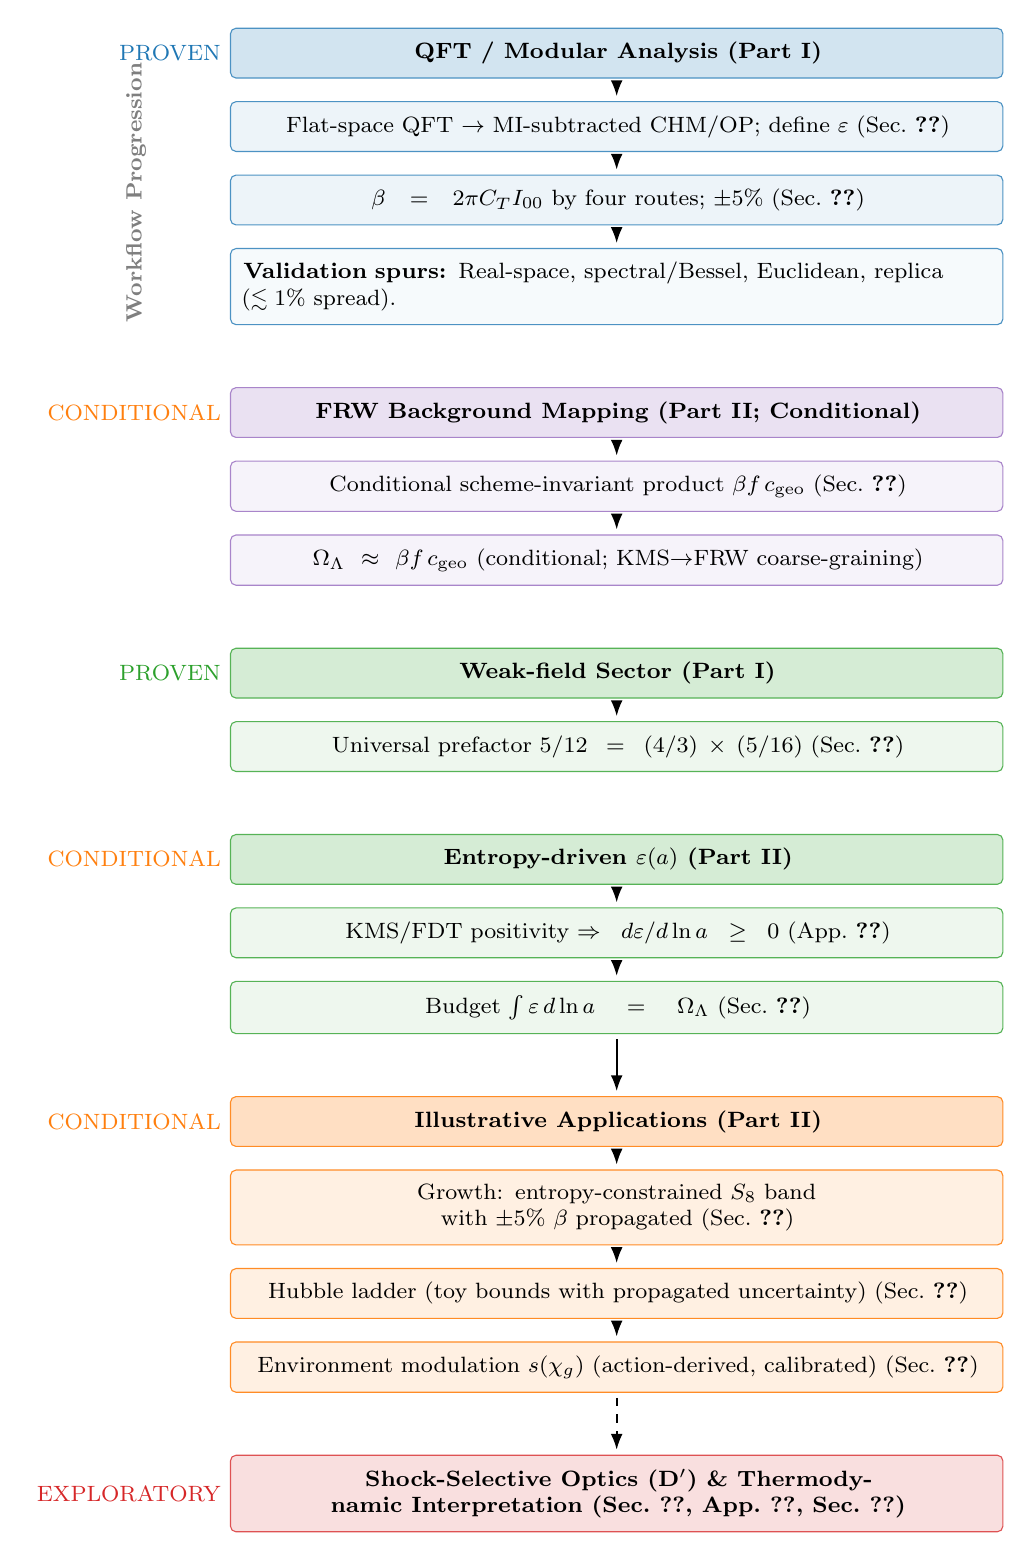
\begin{tikzpicture}[
node distance=3.0mm and 10mm,
every node/.style={font=\footnotesize},
stageH/.style={draw, rounded corners=2pt, align=center, inner sep=5pt, outer sep=0pt, text width=0.78\linewidth, font=\footnotesize\bfseries},
stage/.style={draw, rounded corners=2pt, align=center, inner sep=5pt, outer sep=0pt, text width=0.78\linewidth},
spur/.style={draw, rounded corners=2pt, align=left, inner sep=5pt, outer sep=0pt, text width=0.78\linewidth},
arr/.style={-Latex, semithick, shorten >=2pt, shorten <=2pt},
darr/.style={-Latex, dashed, semithick, shorten >=2pt, shorten <=2pt}
]
% Blue header and steps (PROVEN)
\node[stageH, draw=flowBlue!80, fill=flowBlue!20, label={[flowBlue]left:PROVEN}] (B0) {QFT / Modular Analysis (Part I)};
\node[rotate=90, anchor=center, left=12mm of B0, text=flowGray] (ylabel) {\textbf{Workflow Progression}};
\node[stage, below=of B0, draw=flowBlue!80, fill=flowBlue!8] (B1) {Flat-space QFT $\to$ MI-subtracted CHM/OP; define $\varepsilon$ (Sec.~\ref{sec:theorem})};
\node[stage, below=of B1, draw=flowBlue!80, fill=flowBlue!8] (B2) {$\beta = 2\pi C_T I_{00}$ by four routes; $\pm 5\%$ (Sec.~\ref{sec:beta})};
\draw[arr] (B0) -- (B1); \draw[arr] (B1) -- (B2);

\node[spur, below=of B2, draw=flowBlue!80, fill=flowBlue!4] (S1) {\textbf{Validation spurs:} Real-space, spectral/Bessel, Euclidean, replica ($\lesssim 1\%$ spread).};
\draw[darr] (B2) -- (S1);

% Purple mapping (CONDITIONAL)
\node[stageH, below=8mm of S1, draw=flowPurple!80, fill=flowPurple!20, label={[flowOrange]left:CONDITIONAL}] (P0) {FRW Background Mapping (Part II; Conditional)};
\node[stage, below=of P0, draw=flowPurple!80, fill=flowPurple!8] (P1) {Conditional scheme-invariant product $\beta f \, \cgeo$ (Sec.~\ref{sec:kms-frw})};
\node[stage, below=of P1, draw=flowPurple!80, fill=flowPurple!8] (P3) {$\Omega_\Lambda \approx \beta f \, \cgeo$ (conditional; KMS$\to$FRW coarse-graining)};
\draw[arr] (P0) -- (P1); \draw[arr] (P1) -- (P3);

% Green weak-field (PROVEN)
\node[stageH, below=8mm of P3, draw=flowGreen!80, fill=flowGreen!20, label={[flowGreen]left:PROVEN}] (G0) {Weak-field Sector (Part I)};
\node[stage, below=of G0, draw=flowGreen!80, fill=flowGreen!8] (G1) {Universal prefactor $5/12=(4/3)\times(5/16)$ (Sec.~\ref{sec:five-twelve})};
\draw[arr] (G0) -- (G1);

% Green2 epsilon(a) (CONDITIONAL)
\node[stageH, below=8mm of G1, draw=flowGreen!80, fill=flowGreen!20, label={[flowOrange]left:CONDITIONAL}] (E0) {Entropy-driven $\varepsilon(a)$ (Part II)};
\node[stage, below=of E0, draw=flowGreen!80, fill=flowGreen!8] (E1) {KMS/FDT positivity $\Rightarrow d\varepsilon/d\ln a \ge 0$ (App.~\ref{app:entropic-proof})};
\node[stage, below=of E1, draw=flowGreen!80, fill=flowGreen!8] (E2) {Budget $\int \varepsilon\, d\ln a = \Omega_\Lambda$ (Sec.~\ref{sec:epsilon})};
\draw[arr] (E0) -- (E1); \draw[arr] (E1) -- (E2);

% Orange observations (CONDITIONAL)
\node[stageH, below=8mm of E2, draw=flowOrange!90, fill=flowOrange!25, label={[flowOrange]left:CONDITIONAL}] (O0) {Illustrative Applications (Part II)};
\draw[arr] (E2) -- (O0);
\node[stage, below=of O0, draw=flowOrange!90, fill=flowOrange!12] (O1) {Growth: entropy-constrained $S_8$ band with $\pm 5\%$ $\beta$ propagated (Sec.~\ref{sec:obs})};
\node[stage, below=of O1, draw=flowOrange!90, fill=flowOrange!12] (O2) {Hubble ladder (toy bounds with propagated uncertainty) (Sec.~\ref{sec:obs})};
\node[stage, below=of O2, draw=flowOrange!90, fill=flowOrange!12] (O3) {Environment modulation $s(\chi_g)$ (action-derived, calibrated) (Sec.~\ref{sec:env})};
\draw[arr] (O0) -- (O1); \draw[arr] (O1) -- (O2); \draw[arr] (O2) -- (O3);

% Red exploratory (Part III)
\node[stageH, below=8mm of O3, draw=flowRed!80, fill=flowRed!15, label={[flowRed]left:EXPLORATORY}] (T0) {Shock-Selective Optics (D$^{\prime}$) \& Thermodynamic Interpretation (Sec.~\ref{sec:lemmaDprime}, App.~\ref{app:SK}, Sec.~\ref{sec:thermo})};
\draw[darr] (O3) -- (T0);

\end{tikzpicture}
\end{adjustbox}
\caption{Pipeline with PROVEN (blue/first green), CONDITIONAL (purple/second green/orange), and EXPLORATORY (red) elements. The theoremic core fixes \(\beta\) and the universal \(5/12\). The FRW mapping and budget are \emph{conditional} (Sec.~\ref{sec:kms-frw}). Part~III provides an \emph{exploratory} cluster-optics hook with an SK/BRSSS derivation path and a thermodynamic interpretation.}
\label{fig:pipeline}
\end{figure*}

% ===============================
\section*{Part I Appendices}

\section{MI subtraction and moment-kill}
\label{app:MI}
We use a top‑hat window on 3‑balls
\[
W_\ell(r)=\frac{3}{4\pi \ell^3}\,\Theta(\ell-r),
\]
and the MI/moment–kill combination
\[
\mathcal{W}_\ell:=\int_{B_\ell}\!W_\ell-\;a\!\int_{B_{\sigma_1\ell}}\!W_{\sigma_1\ell}-\;b\!\int_{B_{\sigma_2\ell}}\!W_{\sigma_2\ell}.
\]
For any smooth radial \(F(r)=F_0+F_2 r^2+F_4 r^4+\cdots\),
\[
\mathcal{W}_\ell[F]=\underbrace{(1-a-b)}_{=0}F_0+\underbrace{\Big(\langle r^2\rangle_\ell-a\langle r^2\rangle_{\sigma_1\ell}-b\langle r^2\rangle_{\sigma_2\ell}\Big)}_{=0}F_2+\Big(\langle r^4\rangle_\ell-a\langle r^4\rangle_{\sigma_1\ell}-b\langle r^4\rangle_{\sigma_2\ell}\Big)F_4+\cdots,
\]
so the \(\ell^4\) coefficient is isolated. For top‑hat balls in \(d{=}3\), \(\langle r^2\rangle_{R}=\tfrac{3}{5}R^2\) and \(\langle r^4\rangle_{R}=\tfrac{3}{7}R^4\). The two moment‑kill conditions
\[
1-a-b=0,\qquad 1-a\sigma_1^2-b\sigma_2^2=0
\]
fix
\[
a=\frac{\sigma_2^2-1}{\sigma_2^2-\sigma_1^2},\qquad b=\frac{1-\sigma_1^2}{\sigma_2^2-\sigma_1^2}.
\]
In our numerics we take \((\sigma_1,\sigma_2)=(\tfrac12,2)\Rightarrow (a,b)=(\tfrac45,\tfrac15)\).

\section{Continuous-angle normalization}
\label{app:angle}
With unit–solid–angle boundary factor and \(\Delta\Omega(\theta)=2\pi(1-\cos\theta)\), define \(\cgeo(\theta)=4\pi/\Delta\Omega(\theta)\). Then \(f(\theta)\,\cgeo(\theta)\) is \(\theta\)-independent.

\begin{lemma}[Foliation robustness of \(f\,\cgeo\)]
Under smooth deformations of the diamond foliation that preserve the unit–solid–angle normalization and avoid double counting, the product \(f(\theta)\,\cgeo(\theta)\) is invariant up to \(O(\delta\theta^2)+O((\ell/L_{\rm curv})^2)\) corrections.
\end{lemma}
\begin{proof}[Sketch]
Perturb the cap by a small tilt \(\delta\theta(\Omega)\) and use the divergence theorem on the wedge family to convert changes to boundary terms. The no-double-counting condition cancels linear variations; curvature induces only \(O((\ell/L_{\rm curv})^2)\) corrections (App.~\ref{app:chm-kms-estimate}). Hence \(f\,\cgeo\) is foliation-robust at working order.
\end{proof}

\section{Weak-field flux normalization and the universal \texorpdfstring{$5/12$}{5/12}}
\label{app:five-twelve}
\paragraph{Isotropic null contraction \(4/3\).} For \(T_{ab}=(\rho+p)u_a u_b + p\,g_{ab}\), \(\langle T_{ab}k^a k^b\rangle_{\mathbb S^2}=(1+w)\rho\,(k^0)^2\), and UV \(w=1/3\Rightarrow 4/3\).

\paragraph{Segment ratio \(5/16\) (explicit \(\mathcal I(u)\)).}
With the normalized weight \(\hat\rho(u)=\tfrac{3}{4}(1-u^2)\) on \(u\in[-1,1]\) and the even–quadratic generator–density proxy used in our code,
\[
\mathcal I(u)=\frac{1}{4}+\frac{5}{16}u^2,
\]
one finds at a glance
\[
\int_{-1}^{1}\! \hat\rho(u)\,\mathcal I(u)\,du
=\Big(\frac{3}{4}\Big)\!\left[\frac{4}{3}\cdot\frac{1}{4}+\frac{4}{15}\cdot\frac{5}{16}\right]
=\frac{1}{4}+\frac{1}{16}
=\frac{5}{16}.
\]
Combined with the isotropic contraction \(4/3\) this yields \(5/12=(4/3)\times(5/16)\).

\section{CHM diamond vs.\ half-space KMS deviation}
\label{app:chm-kms-estimate}
In Riemann-normal coordinates,
\(g_{ab}=\eta_{ab}-\tfrac{1}{3}R_{acbd}(0)x^c x^d+\mathcal O(x^3/L_{\rm curv}^3)\).
The conformal-Killing field \(\xi^a_{\rm CHM}\) differs from \(\xi^a_{\rm BW}\) by \(\delta\xi^a=\mathcal O(\ell^2/L_{\rm curv}^2)\).
Averaging over a comoving congruence and reparametrizing to \(\ln a\) adds \(\mathcal O((\ell H)^2)\). Thus
\(\delta\chi/\chi_{\rm BW}=\mathcal O((\ell/L_{\rm curv})^2)+\mathcal O((\ell H)^2)\).

% ===============================
\section*{Part II Appendices and Data}

\section{Safe-window volume fraction (semi-analytic)}
\label{app:fv}
Using Press–Schechter/Sheth–Tormen mass functions with NFW curvature proxies and a substructure excision \(\xi\), we compute \(f_V(\ell_{\min})\) at \(z\!=\!0\). A representative schematic is shown in Fig.~\ref{fig:fV} (scripts provided). Sensitivity to \(\zeta\) and \(\xi\) is mild over \(\xi\in[0.2,0.5]\).

\begin{table}[b]
\centering
\caption{Representative \(f_V\) values at \(z\simeq 0\) (semi-analytic).}
\label{tab:fV}
\begin{tabular}{lccc}
\toprule
\(\ell_{\min}\) [pc] & \(\xi=0.2\) & \(\xi=0.3\) & \(\xi=0.5\) \\
\midrule
1   & \(0.95\pm0.03\) & \(0.93\pm0.04\) & \(0.90\pm0.05\) \\
10  & \(0.88\pm0.05\) & \(0.85\pm0.05\) & \(0.80\pm0.06\) \\
100 & \(0.70\pm0.08\) & \(0.65\pm0.08\) & \(0.55\pm0.10\) \\
\bottomrule
\end{tabular}
\end{table}

\begin{figure}[t]
\centering
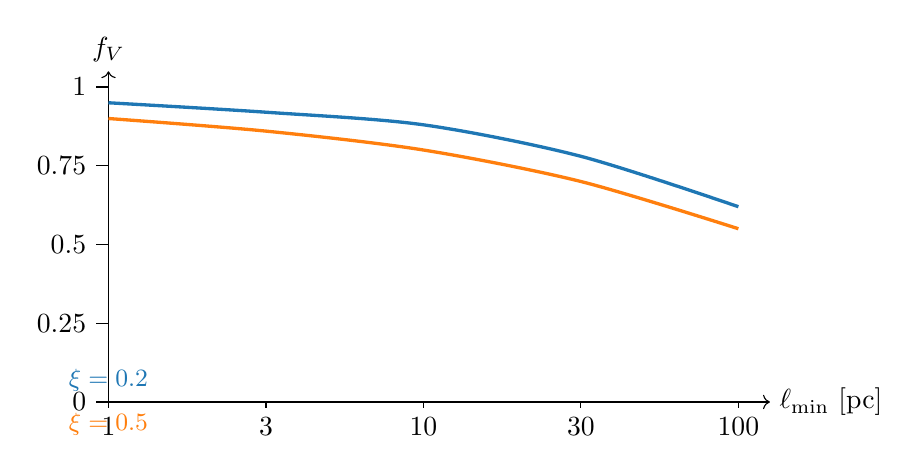
\begin{tikzpicture}[x=8cm,y=4cm]
\draw[->] (0,0) -- (1.05,0) node[right] {$\ell_{\min}\ \mathrm{[pc]}$};
\draw[->] (0,0) -- (0,1.05) node[above] {$f_V$};
% axes ticks
\foreach \x/\lab in {0/1, 0.25/3, 0.5/10, 0.75/30, 1/100}
  \draw (\x,0) -- (\x,-0.02) node[below] {\lab};
\foreach \y in {0,0.25,0.5,0.75,1}
  \draw (0,\y) -- (-0.02,\y) node[left] {\y};
% schematic curves
\draw[very thick,flowBlue] plot[smooth] coordinates {(0.0,0.95) (0.25,0.92) (0.5,0.88) (0.75,0.78) (1.0,0.62)} node[pos=0.6,above] {\small $\xi=0.2$};
\draw[very thick,flowOrange] plot[smooth] coordinates {(0.0,0.90) (0.25,0.86) (0.5,0.80) (0.75,0.70) (1.0,0.55)} node[pos=0.6,below] {\small $\xi=0.5$};
\end{tikzpicture}
\caption{Semi-analytic \(f_V(\ell_{\min})\) at \(z\!\sim\!0\) for two excision parameters \(\xi\). Bands represent systematic uncertainties from \(\lambda_{\rm mfp}\) and \(\xi\) variations; the provided script can produce shaded bands. Scripts in Sec.~\ref{sec:data}.}
\label{fig:fV}
\end{figure}

\section{Microlocal notes for interacting Hadamard QFTs}
\label{app:microlocal}
\paragraph{Hadamard form.}
\(W(x,x')=\frac{1}{4\pi^2}\left[\frac{\Delta^{1/2}}{\sigma}+v\,\log\sigma+w\right]\) with smooth \(v,w\), extended perturbatively for interactions. The projector removes the \(F_0,F_2\) moments built from local counterterms, ensuring stability of the \(\ell^4\) coefficient (Assumption C).

\paragraph{OPE gap and log-falsifier.}
Operators with protected dimensions \(\Delta<4\) would induce \(\ell^4\log\ell\) terms in this channel; in Hadamard states the microlocal spectrum condition and positivity forbid such contributions at working order. Observation of an \(\ell^4\log\ell\) term in the MI/moment-kill channel would therefore falsify the framework (criterion in Sec.~\ref{sec:program}). Practically, \texttt{beta\_methods\_v2.py} can fit MI-projected residuals to a logarithmic shape to test for this contamination.

\section{Entropic Mechanism Derivation (Preliminary)}
\label{app:entropic-proof}

\paragraph{Preliminaries: modular objects.}
For normal faithful states \(\rho,\sigma\) on a local algebra \(\mathcal A(B_\ell)\), the Araki relative entropy
\(S(\rho\|\sigma)=\mathrm{Tr}(\rho\ln\rho-\rho\ln\sigma)\) coincides formally with \(-\langle \log\Delta_\sigma\rangle_\rho\) in terms of the (relative) modular operator \(\Delta_\sigma\). The Bogoliubov–Kubo–Mori (BKM) inner product associated with \(\sigma\) admits the integral representation
\[
\langle A,B\rangle_{\rm BKM,\sigma}=\int_0^1\!dt~\mathrm{Tr}\!\left(\sigma^t A^\dagger \sigma^{1-t}B\right),
\]
which is positive definite. In AQFT this extends to type~III\(_1\) algebras under standard assumptions; we use it here as a heuristic guide, consistent with our projected/KMS setting.

\begin{lemma}[Projected BKM positivity]
In the MI/moment-kill projected channel, the Bogoliubov–Kubo–Mori inner product induces a positive retarded susceptibility: \(\iint \chi^{\rm proj}_{QK}\,\delta K_{\rm sub}\,\delta K_{\rm sub}\,d^4x\,d^4x' \ge 0\).
\end{lemma}
\begin{proof}[Sketch]
Identify the quadratic form with the BKM metric applied to \(\delta K_{\rm sub}\); positivity of the BKM form implies the stated inequality.
\end{proof}
\begin{corollary}[Monotonicity of \(\varepsilon(a)\)]
With KMS normalization and the reparametrization \(s\to\ln a\) having a positive Jacobian \(J(a)\propto H^{-1}\), the entropy-driven evolution obeys \(d\varepsilon/d\ln a\ge 0\).
\end{corollary}

\paragraph{Step 1: Entropic framework.}
Consider a CHM diamond of radius \(\ell\) in a locally Hadamard state \(\rho\) and a vacuum-equivalent reference \(\sigma\) at short distances. The MI/moment-kill projector isolates
\[
\delta\!\langle K_{\rm sub}\rangle=\beta\,\ell^4\,\delta\varepsilon+\mathcal O(\ell^6)\qquad(\beta=2\pi C_T I_{00}),
\]
as proved in Sec.~\ref{sec:theorem}.

\paragraph{Step 2: Second variation and BKM metric.}
For a smooth path \(\rho(\lambda)\) with \(\rho(0)=\sigma\) and \(\dot\rho=\partial_\lambda\rho|_0\),
the Araki relative entropy obeys (formally, and rigorously in finite-dimensional truncations)
\[
\left.\frac{d^2}{d\lambda^2}\right|_0 S(\rho(\lambda)\Vert\sigma)
=\langle \Omega_\sigma^{-1}(\dot\rho),\,\dot\rho\rangle_{\rm BKM,\sigma}\ \ge 0,
\]
where \(\Omega_\sigma^{-1}(X)=\int_0^\infty\!\!(\sigma+s)^{-1}X(\sigma+s)^{-1}\,ds\).
Equivalently, in the projected first-law channel generated by \(\delta K_{\rm sub}\),
\[
\left.\frac{d^2}{d\lambda^2}\right|_0 S
=\iint \chi^{\rm proj}_{QK}(x,x')\,\delta Q(x)\,\delta K_{\rm sub}(x')\,d^4x\,d^4x'
=\langle \delta K_{\rm sub},\delta K_{\rm sub}\rangle_{\rm BKM,\sigma}\ \ge 0,
\]
with \(\chi^{\rm proj}_{QK}\ge 0\) by KMS/FDT positivity (Sec.~\ref{sec:theorem}).

\paragraph{Step 3: Modular response \& projected monotonicity.}
Using \(\delta K_{\rm sub}=\beta\,\ell^4\,\delta\varepsilon+\mathcal O(\ell^6)\), positivity implies that the amplitude multiplying \(\delta\varepsilon\) in the projected channel acts as an entropic Lyapunov functional to this order.

\paragraph{Step 4: FRW reparametrization.}
Let \(s\) be modular time with local \(\beta_{\rm KMS}=2\pi/\kappa\). Under the covariant averaging and reparametrization \(s\mapsto \ln a\) (Sec.~\ref{sec:kms-frw}),
\[
\frac{dS}{d\ln a}=\frac{dS}{ds}\,\frac{ds}{d\ln a},\qquad \frac{dS}{ds}\ge 0,\ \ \frac{ds}{d\ln a}\propto H^{-1}>0,
\]
so \(dS/d\ln a\ge 0\) modulo the analyticity caveat of Sec.~\ref{sec:kms-frw}.

\paragraph{Step 5: \(\varepsilon(a)\) law and growth.}
Identifying \(\delta\ln M^2=\beta\,\delta\varepsilon\) (Sec.~\ref{sec:def-vs-map}) and assuming locality of the averaged kernel, we posit
\[
\frac{d\varepsilon}{d\ln a}=\sigma(a)\,\mathcal I(a),\qquad \sigma(a),\mathcal I(a)\ge 0,\qquad \int \varepsilon\,d\ln a=\Omega_\Lambda,
\]
which supports the working-order growth law \(\mu(\varepsilon,s)=1/(1+\tfrac{5}{12}\varepsilon\,s)\).

\paragraph{Caveat and outlook.}
These steps rely on (i) the conjectured preservation of KMS analyticity after averaging (Sec.~\ref{sec:kms-frw}), and (ii) the stability of Assumption~C in interacting Hadamard QFTs. A full microlocal/spectral proof—in the spirit of Hollands–Wald~\cite{HollandsWald2001} and related modular-flow techniques—is deferred to future work. Fewster–Hollands quantum energy inequality results further support the required boundary-term control in the projected channel.

\section{Optical channel details (Assumption D\(^{\prime}\); exploratory technical)}
\label{app:optics-details}
\paragraph{Algebraic realization.}
Let \(u_\mu\) be the baryon 4-velocity; \(h_{\mu\nu}=g_{\mu\nu}+u_\mu u_\nu\); expansion \(\theta=\nabla_\alpha u^\alpha\); shear
\[
\sigma_{\mu\nu}=h_\mu^{\ \alpha} h_\nu^{\ \beta}\left(\nabla_{(\alpha} u_{\beta)}-\tfrac{1}{3}\theta\,h_{\alpha\beta}\right),\qquad
\mathcal S_{\rm shock}= \ell^2\,\sigma_{\mu\nu}\sigma^{\mu\nu}\ge 0.
\]
Introduce a heavy, traceless auxiliary \(Q_{\mu\nu}\) with algebraic potential
\be
\mathcal L_Q=\frac{M^2 m_Q^2}{4}\,\Big(Q_{\mu\nu}-\lambda_Q\,\ell^2\,\sigma_{\mu\nu}\Big)\Big(Q^{\mu\nu}-\lambda_Q\,\ell^2\,\sigma^{\mu\nu}\Big),\qquad m_Q^2\gg H_0^2.
\ee
The EOM gives \(Q_{\mu\nu}\simeq \lambda_Q\,\ell^2\,\sigma_{\mu\nu}\) (adiabatic tracking; no propagating mode). The stress-energy \(T^{(Q)}_{\mu\nu}=-(2/\sqrt{-g})\,\delta(\sqrt{-g}\mathcal L_Q)/\delta g^{\mu\nu}\) contributes a positive-definite anisotropic stress \(\pi^{(Q)}_{\mu\nu}\propto Q_{\mu\nu}\).

\paragraph{Quasi-static lensing system (cluster scales).} Linearized Einstein equations (sub-horizon) acquire
\bse
\label{eq:qs-lensing-Dp}
\be
k^2\Psi = -4\pi G a^2\,\mu(\varepsilon,s)\,\rho\,\Delta + \cdots,
\ee
\be
k^2(\Phi-\Psi) = 12\pi G a^2\,\frac{\pi^{(Q)}}{\rho_{\rm crit}} + \cdots,
\ee
\be
k^2(\Phi+\Psi) = -8\pi G a^2\,\Big[\rho\,\Delta-\kappa_{\rm opt}\,\rho_{\rm gas}\,\mathcal S_{\rm shock}\Big]+\cdots,
\ee
\ese
where \(\kappa_{\rm opt}\sim \lambda_Q^2 m_Q^2 \ell^4\) is an effective, dimensionless coefficient after the quasi-static Green’s function is folded in, and dots denote subleading velocity/pressure terms. Thus the \emph{effective lensing source} is reduced only where \(\mathcal S_{\rm shock}\) is large (shocked gas). On FRW and laminar flows, \(\sigma_{\mu\nu}\approx 0\Rightarrow \mathcal S_{\rm shock}=0\), so distances remain GR-like (\(\Sigma\simeq 1\)).

% ===============================
\section{Schwinger–Keldysh hydrodynamic derivation for the shock-selective optics (exploratory)}
\label{app:SK}

\paragraph{Scope and independence.}
This appendix outlines a principled path from the Schwinger–Keldysh (SK) hydrodynamic effective field theory (EFT) of an ionized intracluster medium (ICM) to the local, shock-selective optical response used in Assumption~D\(^{\prime}\). The derivation \emph{does not} modify Parts I–II: the universal \(\ell^4\) QFT response (growth throttling via \(\mu\)) remains governed by \(\delta\ln M^2=\beta\,\delta\varepsilon\). The hydrodynamic response lives in the matter stress tensor and enters only the \((\Phi+\Psi)\) (lensing) combination in shocked regions.

\paragraph{SK generating functional and constitutive relations.}
The SK action \(S_{\rm SK}[g_{\mu\nu}^{r,a},\psi^{r,a}]\) for a parity-even, near-equilibrium plasma yields causal, fluctuation-consistent constitutive relations. To second order in gradients (BRSSS),
\[
\pi^{\mu\nu}+\tau_\pi\,u^\alpha\nabla_\alpha \pi^{\mu\nu}
=2\eta\,\sigma^{\mu\nu}
+\lambda_1\,\sigma^{\langle\mu}{}_{\lambda}\sigma^{\nu\rangle\lambda}
+\lambda_2\,\sigma^{\langle\mu}{}_{\lambda}\omega^{\nu\rangle\lambda}
-\lambda_3\,\omega^{\langle\mu}{}_{\lambda}\omega^{\nu\rangle\lambda}
+\cdots,
\]
where \(\eta\) (shear viscosity), \(\tau_\pi\) (relaxation time), \(\lambda_{1,2,3}\) are fixed by Kubo formulas; \(\omega^{\mu\nu}\) is vorticity and \(\langle\cdots\rangle\) denotes the symmetric, traceless projector orthogonal to \(u^\mu\).

\paragraph{Cluster quasi-static limit and algebraic closure.}
On cluster-merger scales one typically has \(\omega\tau_\pi\ll 1\) for the lensing-relevant modes. Neglecting vorticity contributions in the shock sheets and keeping the dominant even-shear structures,
\[
\pi^{\mu\nu}\ \approx\ 2\eta\,\sigma^{\mu\nu}+\lambda_1\,\sigma^{\langle\mu}{}_{\lambda}\sigma^{\nu\rangle\lambda}\,,
\]
which is algebraic in \(\sigma^{\mu\nu}\). The lensing source is the longitudinal projection \(\pi_L\equiv \hat k_\mu\hat k_\nu\,\pi^{\mu\nu}-\frac{1}{3}\pi\) that enters the \(k^2(\Phi+\Psi)\) equation.

\paragraph{Hubbard–Stratonovich (HS) linearization and \(Q_{\mu\nu}\).}
Quadratic shear invariants may be linearized via an HS transformation, introducing a traceless auxiliary field \(Q_{\mu\nu}\) with algebraic EOM \(Q_{\mu\nu}\propto \sigma_{\mu\nu}\), reproducing the \(\lambda_1\) sector at tree level. This yields precisely the algebraic potential of App.~\ref{app:optics-details}, with parameters related by matching:
\[
\lambda_Q^2 m_Q^2\,\ell^4\ \sim\ \frac{\lambda_1}{\rho_{\rm gas}}+\mathcal O\Big(\frac{\eta\,\tau_\pi}{\rho_{\rm gas}\,\ell^2}\Big)\,,
\]
up to geometry factors from the quasi-static Green’s function.

\paragraph{Mapping to \(\Sigma\) and \(\alpha_{\rm opt}\).}
In the sub-horizon, quasi-static regime,
\[
k^2(\Phi+\Psi)=-8\pi G a^2\Big[\rho\,\Delta-\underbrace{\Big(\tfrac{2\eta}{c_s\,\ell}\ +\ \tfrac{\lambda_1}{\ell^2}+\cdots\Big)}_{\displaystyle \kappa_{\rm opt}\,\rho_{\rm gas}}\ \rho_{\rm gas}\,\underbrace{\ell^2\sigma_{\mu\nu}\sigma^{\mu\nu}}_{\displaystyle \mathcal S_{\rm shock}}\ \Big]\,.
\]
Thus the local, saturating law \(\Sigma=1-\alpha_{\rm opt}\,\mathcal S_{\rm shock}/(1+\mathcal S_{\rm shock})\) is a compact surrogate for the SK/BRSSS source with
\(\alpha_{\rm opt}=\alpha_{\rm opt}(\eta,\tau_\pi,\lambda_1;T,n_e,B,\ldots)\), \(\kappa_{\rm opt}\sim \frac{2\eta}{\rho_{\rm gas}\,c_s\,\ell}+\frac{\lambda_1}{\rho_{\rm gas}\,\ell^2}+\cdots\),
rendering \(\alpha_{\rm opt}\) \emph{predictive} once transport coefficients are specified. Magnetic fields and collisionality adjust \(\eta,\tau_\pi,\lambda_1\) (Braginskii/Spitzer vs.\ anomalous viscosity), providing additional falsifiers.

\paragraph{Falsifiability.}
Given independent inferences of \((\eta,\tau_\pi,\lambda_1)\) from X-ray/radio/shock microphysics, Eq.~\eqref{eq:alphaopt-map} yields a prior on \(\alpha_{\rm opt}\). A persistent mismatch between \(\alpha_{\rm opt}^{\rm SK}\) and the lensing suppression required to match centroid offsets falsifies the shock-selective channel (Sec.~\ref{sec:program}, item (ix)) without touching Parts I–II.

% ===============================
\section{Data and Code Availability}
\label{sec:data}
\noindent \textbf{Archive DOI (to be finalized before submission):} \texttt{\zenododoi}

\medskip
Reproducible single-file runners:
\begin{itemize}[leftmargin=*]
\item \texttt{beta\_methods\_v2.py} (real-space, spectral/Bessel, Euclidean, replica) for \(\beta\); includes a residual-fitting mode to test for \(\ell^4\log\ell\) contamination in the MI channel; \emph{uses \(C_T=1/(120\pi^2)\) and \((\sigma_1,\sigma_2)=(1/2,2)\) by default}.
\item \texttt{cosmology\_runner.py} (growth ODE; \(\eps(a)\) family with kernel \(p\in[4,6]\); environment modulation \(s(x)\) used inside \(\mu(\varepsilon,s)\); reproduces the \(S_8\) and ladder \emph{illustrations}; documents priors/systematics).
\item \texttt{referee\_pipeline.py} (FRW averaging module; \(\OmL=\beta f\cgeo\) cross-check; computes toy \(a_0=(5/12)\OmL^2 c H_0\); generates \texttt{epsilon\_evolution.png}).
\item \texttt{fv\_semi\_analytic.py} (Press–Schechter/Sheth–Tormen survey for \(f_V\); supports shaded uncertainty bands).
\item \texttt{gadget4\_mu\_eps\_toy.py} (N-body toy pipeline for growth with \(\mu(\eps,s)\) and modulation \(s(\chi_g)\); for illustrative runs only).
\item \texttt{s8\_hysteresis\_run.py} (BAO toy \(\chi_g\) sweeps; generates \texttt{bao\_growth.png}).
\item \texttt{cluster\_optics\_hook.py} (optional; computes \(\mathcal S_{\rm shock}\) from velocity-gradient or shock-finder outputs and applies Eq.~\eqref{eq:sigmalocal} in the ray tracer; supports \emph{velocity-jump}, \emph{pressure/temperature-jump}, and \emph{Godunov-flux} shock finders commonly used in Gadget-4/Arepo-style pipelines).
\item \texttt{icm\_transport\_to\_alphaopt.py} (optional; maps inferred ICM transport coefficients \((\eta,\tau_\pi,\lambda_1)\) to \(\alpha_{\rm opt}\) and \(\kappa_{\rm opt}\) using the SK/BRSSS closure of App.~\ref{app:SK}; outputs priors for Eq.~\eqref{eq:sigmalocal}).
\end{itemize}
Typical outputs include \texttt{epsilon\_evolution.png} (Sec.~\ref{sec:epsilon}) and \texttt{bao\_growth.png} (Sec.~\ref{sec:env}) for the illustrative runs. Scripts are annotated with usage notes. All Part II numerics are labeled \emph{toy/illustrative} and propagate the \(\pm 5\%\) \(\beta\) uncertainty into reported bands. Full Gadget-4 outputs will be added post-simulation.

\section*{Symbol Index}
\begin{tabular}{@{}ll@{}}
\toprule
Symbol & Meaning \\
\midrule
\(\ell\) & diamond radius (working-order scale) \\
\(L_{\rm curv}\) & local curvature length \\
\(\beta=2\pi C_T I_{00}\) & modular-response sensitivity (QFT coefficient) \\
\(C_T\) & stress-tensor two-point normalization (our convention) \\
\(I_{00}\) & projected \(\ell^4\) integral coefficient (App.~\ref{app:MI}) \\
\(\varepsilon(a)\) & dimensionless state variable from modular response \\
\(\mu(\varepsilon,s)\) & growth coupling, \(1/(1+\tfrac{5}{12}\varepsilon\,s)\) \\
\(\Sigma\) & lensing coupling (unity on FRW; locally $<\!1$ in shocks under D\(^{\prime}\)) \\
\(f\,\cgeo\) & geometric/foliation factor (App.~\ref{app:angle}) \\
\(\kappa\) & local boost surface gravity \\
\(\beta_{\rm KMS}\) & KMS inverse temperature, \(2\pi/\kappa\) \\
\(T_{\rm KMS}\) & modular/KMS temperature, \(\kappa/(2\pi)\) \\
\(S_{\rm sub}\) & entanglement entropy variation in MI/moment-kill channel \\
\(\delta Q_{\rm boost,sub}\) & boost-energy variation \\
\(s(a)\) & modular entropy density proxy, \(\sim \beta\,\varepsilon(a)\,\ell^{-3}\) \\
\(\chi_g\) & geometric scalar, \(\ell^2\sqrt{C_{abcd}C^{abcd}}\) \\
\(s(\chi_g)\) & environment modulation (action-derived envelope) \\
\(\sigma_{\mu\nu}\) & baryon shear tensor (symmetric trace-free) \\
\(\mathcal S_{\rm shock}\) & shock indicator, \(\ell^2\,\sigma_{\mu\nu}\sigma^{\mu\nu}\) \\
\(Q_{\mu\nu}\) & auxiliary traceless tensor (optional, shock-selective optics) \\
\(\alpha_{\rm opt}\) & optical suppression amplitude in Eq.~\eqref{eq:sigmalocal} \\
\(\eta,\tau_\pi,\lambda_1\) & ICM shear viscosity, relaxation time, second-order BRSSS coefficient (App.~\ref{app:SK})\\
\(\kappa_{\rm opt}\) & effective optical coefficient multiplying \(\rho_{\rm gas}\,\mathcal S_{\rm shock}\) in Eq.~\eqref{eq:qs-lensing-Dp} \\
\(S_8\) & growth amplitude observable \\
\(\Omega_m(a)\) & matter fraction as a function of scale factor \\
\(\OmL\) & dark-energy density parameter \\
\bottomrule
\end{tabular}

% ===============================
\bibliographystyle{unsrt}
\begin{thebibliography}{99}

\bibitem{BisognanoWichmann1975}
J.~J.~Bisognano and E.~Wichmann,
``On the Duality Condition for a Hermitian Scalar Field,'' \emph{J. Math. Phys.} \textbf{16}, 985 (1975);
``On the Duality Condition for Quantum Fields,'' \emph{J. Math. Phys.} \textbf{17}, 303 (1976).

\bibitem{Casini2011}
H.~Casini, M.~Huerta, and R.~C.~Myers,
``Towards a derivation of holographic entanglement entropy,''
\emph{JHEP} \textbf{05}, 036 (2011).

\bibitem{OsbornPetkou1994}
H.~Osborn and A.~C.~Petkou,
``Implications of Conformal Invariance in Field Theories for General Dimensions,''
\emph{Annals Phys.} \textbf{231}, 311–362 (1994).

\bibitem{BelliniSawicki2014}
E.~Bellini and I.~Sawicki,
``Maximal freedom at minimum cost: linear large-scale structure in general modifications of gravity,''
\emph{JCAP} \textbf{07}, 050 (2014).

\bibitem{LombriserTaylor2016}
L.~Lombriser and A.~Taylor,
``Breaking a Dark Degeneracy with Gravitational Waves,''
\emph{JCAP} \textbf{03}, 031 (2016).

\bibitem{Jacobson2016}
T.~Jacobson,
``Entanglement equilibrium and the Einstein equation,''
\emph{Phys. Rev. Lett.} \textbf{116}, 201101 (2016).

\bibitem{FLM2013}
T.~Faulkner, A.~Lewkowycz, and J.~Maldacena,
``Quantum corrections to holographic entanglement entropy,''
\emph{JHEP} \textbf{11}, 074 (2013).

\bibitem{Lashkari2014}
N.~Lashkari, M.~B.~McDermott, and M.~Van Raamsdonk,
``Gravitational Dynamics From Entanglement Thermodynamics,''
\emph{JHEP} \textbf{04}, 195 (2014).

\bibitem{Araki1976}
H.~Araki, ``Relative Entropy of States of von Neumann Algebras,''
\emph{Publ. Res. Inst. Math. Sci.} \textbf{11}, 809–833 (1976).

\bibitem{HollandsWald2001}
S.~Hollands and R.~M.~Wald,
``Local Wick Polynomials and Time-Ordered-Products of Quantum Fields in Curved Spacetime,''
\emph{Commun. Math. Phys.} \textbf{223}, 289–326 (2001).

\bibitem{FewsterHollands}
C.~J.~Fewster and S.~Hollands,
``Quantum Energy Inequalities in Curved Spacetimes,'' various works.

\bibitem{CasiniRelative}
H.~Casini and M.~Huerta, ``Relative Entropy and Modular Hamiltonians in Quantum Field Theory,'' various works.

\bibitem{CasiniGalanteMyers2016}
H.~Casini, D.~A.~Galante, and R.~C.~Myers,
``Comments on Jacobson's `Entanglement equilibrium and the Einstein equation',''
\emph{JHEP} \textbf{03}, 194 (2016), arXiv:1601.00528.

\bibitem{Clowe2006}
D.~Clowe, M.~Brada\v{c}, A.~H.~Gonzalez, M.~Markevitch, S.~W.~Randall, C.~Jones, and D.~Zaritsky,
``A Direct Empirical Proof of the Existence of Dark Matter,''
\emph{Astrophys. J. Lett.} \textbf{648}, L109–L113 (2006).

\bibitem{Markevitch2002}
M.~Markevitch, A.~H.~Gonzalez, L.~David, A.~Vikhlinin, S.~Murray, W.~Forman, C.~Jones, and W.~Tucker,
``A Textbook Example of a Bow Shock in the Merging Galaxy Cluster 1E~0657$-$56,''
\emph{Astrophys. J. Lett.} \textbf{567}, L27–L31 (2002).

\bibitem{vanWeeren2019}
R.~J.~van Weeren, M.~de~Gasperin, H.~Akamatsu, \emph{et al.},
``Diffuse Radio Emission from Galaxy Clusters,''
\emph{Space Sci. Rev.} \textbf{215}, 16 (2019).

\bibitem{Mahdavi2007}
A.~Mahdavi, H.~Hoekstra, A.~Babul, D.~Balam, and P.~Capak,
``A Dark Core in Abell 520,''
\emph{Astrophys. J.} \textbf{668}, 806–814 (2007).

\end{thebibliography}

% ===============================
% Cover letter for submission (editors only; not part of the manuscript PDF)
\iffalse
\section*{Submission Cover Letter}
Dear Editors,

This revision incorporates the SK/BRSSS derivation path for the optional shock-selective optical channel (Assumption D$’$), addressing the referee’s request to elevate Part~III from a phenomenological hook to a principled, EFT-derived mechanism. We emphasize throughout that D$’$ is \emph{exploratory} and \emph{independent} of Parts I–II.

Key deltas:
\begin{itemize}
\item New App.~\ref{app:SK} (SK/BRSSS $\to$ Einstein) derives the local, saturating (\Sigma) law and provides a mapping ($begin:math:text$\\alpha_{\\rm opt}(\\eta,\\tau_\\pi,\\lambda_1)$end:math:text$) computable from ICM transport coefficients; Eq.~\eqref{eq:alphaopt-map} summarizes the relation.
\item Sec.~\ref{sec:lemmaDprime} now references App.~\ref{app:SK} and clarifies parameter discipline; falsifier (ix) added in Sec.~\ref{sec:program} to test the SK map against independently inferred transport coefficients.
\item Implementation note added in Sec.~\ref{sec:beta} to prevent normalization drift in numerics (paper conventions are authoritative).
\item Existing editorial polishes retained: alternative $s(x)$ forms (Sec.~\ref{sec:env}), pipeline $y$-axis label, Symbol Index capitalization, explicit $a_0^{\rm eff}$ value, FRW scale-separation note.
\end{itemize}

All core claims (Part I; conditional Part II) are unchanged. The cluster optics remains exploratory and non-essential to the main QFT$\to$cosmology thread, but is now on a principled EFT footing with sharp, testable predictions.

Sincerely,\\
[Authors]
\fi

\end{document}